% Options for packages loaded elsewhere
\PassOptionsToPackage{unicode}{hyperref}
\PassOptionsToPackage{hyphens}{url}
%
\documentclass[
  openany]{book}
\usepackage{lmodern}
\usepackage{amsmath}
\usepackage{ifxetex,ifluatex}
\ifnum 0\ifxetex 1\fi\ifluatex 1\fi=0 % if pdftex
  \usepackage[T1]{fontenc}
  \usepackage[utf8]{inputenc}
  \usepackage{textcomp} % provide euro and other symbols
  \usepackage{amssymb}
\else % if luatex or xetex
  \usepackage{unicode-math}
  \defaultfontfeatures{Scale=MatchLowercase}
  \defaultfontfeatures[\rmfamily]{Ligatures=TeX,Scale=1}
\fi
% Use upquote if available, for straight quotes in verbatim environments
\IfFileExists{upquote.sty}{\usepackage{upquote}}{}
\IfFileExists{microtype.sty}{% use microtype if available
  \usepackage[]{microtype}
  \UseMicrotypeSet[protrusion]{basicmath} % disable protrusion for tt fonts
}{}
\makeatletter
\@ifundefined{KOMAClassName}{% if non-KOMA class
  \IfFileExists{parskip.sty}{%
    \usepackage{parskip}
  }{% else
    \setlength{\parindent}{0pt}
    \setlength{\parskip}{6pt plus 2pt minus 1pt}}
}{% if KOMA class
  \KOMAoptions{parskip=half}}
\makeatother
\usepackage{xcolor}
\IfFileExists{xurl.sty}{\usepackage{xurl}}{} % add URL line breaks if available
\IfFileExists{bookmark.sty}{\usepackage{bookmark}}{\usepackage{hyperref}}
\hypersetup{
  pdftitle={Documento Técnico N°1: Medición del Turismo},
  pdfauthor={Dirección Nacional de Mercados y Estadísticas - Subsecretaría de Desarrollo Estratégico},
  hidelinks,
  pdfcreator={LaTeX via pandoc}}
\urlstyle{same} % disable monospaced font for URLs
\usepackage{longtable,booktabs}
\usepackage{calc} % for calculating minipage widths
% Correct order of tables after \paragraph or \subparagraph
\usepackage{etoolbox}
\makeatletter
\patchcmd\longtable{\par}{\if@noskipsec\mbox{}\fi\par}{}{}
\makeatother
% Allow footnotes in longtable head/foot
\IfFileExists{footnotehyper.sty}{\usepackage{footnotehyper}}{\usepackage{footnote}}
\makesavenoteenv{longtable}
\usepackage{graphicx}
\makeatletter
\def\maxwidth{\ifdim\Gin@nat@width>\linewidth\linewidth\else\Gin@nat@width\fi}
\def\maxheight{\ifdim\Gin@nat@height>\textheight\textheight\else\Gin@nat@height\fi}
\makeatother
% Scale images if necessary, so that they will not overflow the page
% margins by default, and it is still possible to overwrite the defaults
% using explicit options in \includegraphics[width, height, ...]{}
\setkeys{Gin}{width=\maxwidth,height=\maxheight,keepaspectratio}
% Set default figure placement to htbp
\makeatletter
\def\fps@figure{htbp}
\makeatother
\setlength{\emergencystretch}{3em} % prevent overfull lines
\providecommand{\tightlist}{%
  \setlength{\itemsep}{0pt}\setlength{\parskip}{0pt}}
\setcounter{secnumdepth}{5}
  %%% REFERENCIAS
        \usepackage{hyperref}
        % links del indice en negro; citas y URL en azul
        \hypersetup{colorlinks = true, urlcolor={blue}, 
        citecolor={blue}, linkcolor ={black}}
\usepackage[spanish]{babel} % Idiomas en los que se escribe el documento. 
\usepackage{booktabs}
\usepackage{amsthm}

\usepackage[final]{pdfpages}

\makeatletter
\def\thm@space@setup{%
  \thm@preskip=8pt plus 2pt minus 4pt
  \thm@postskip=\thm@preskip
}
\makeatother
\let\oldmaketitle\maketitle
\AtBeginDocument{\let\maketitle\relax}
\ifluatex
  \usepackage{selnolig}  % disable illegal ligatures
\fi
\usepackage[]{natbib}
\bibliographystyle{apalike}

\title{Documento Técnico N°1: Medición del Turismo}
\usepackage{etoolbox}
\makeatletter
\providecommand{\subtitle}[1]{% add subtitle to \maketitle
  \apptocmd{\@title}{\par {\large #1 \par}}{}{}
}
\makeatother
\subtitle{Conceptos y Elementos Básicos para la Medición Provincial de los Turistas}
\author{Dirección Nacional de Mercados y Estadísticas - Subsecretaría de Desarrollo Estratégico}
\date{25 de junio de 2021}

\begin{document}
\maketitle

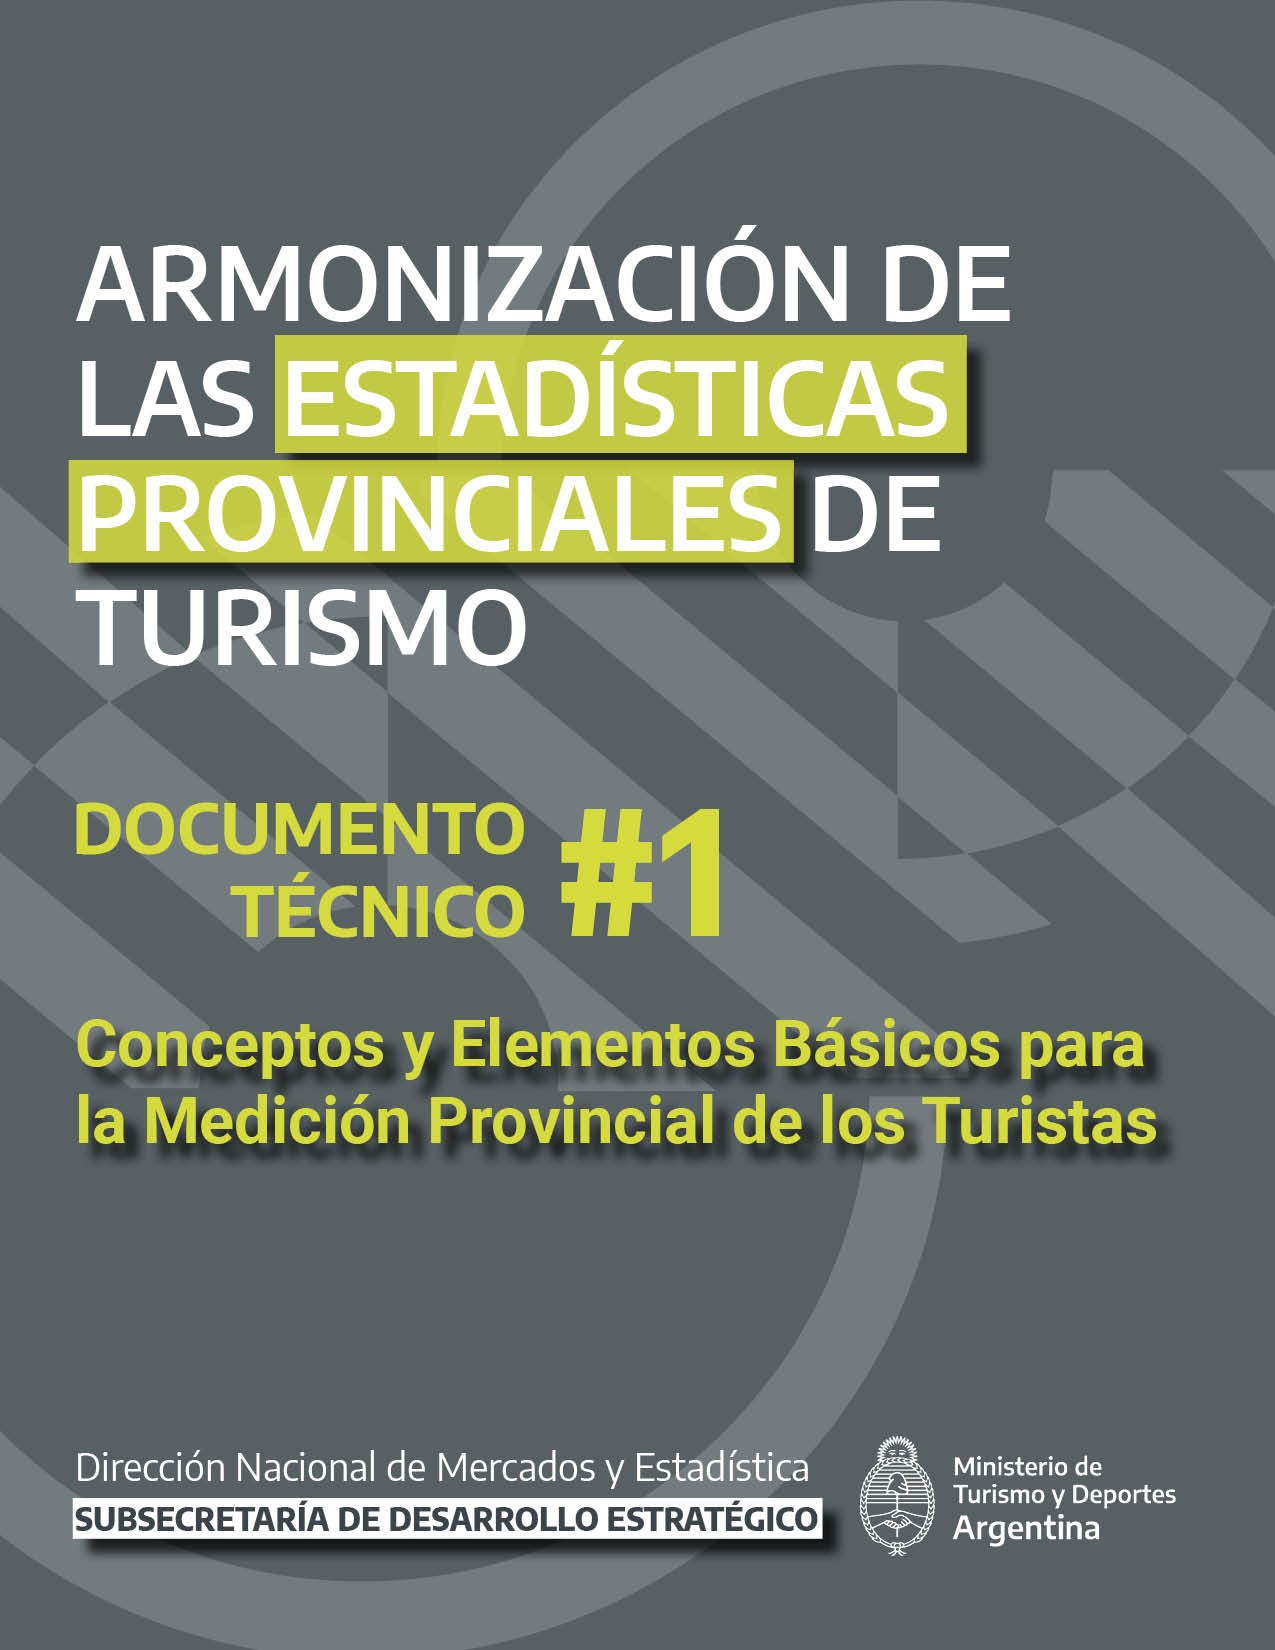
\includepdf[pages={1}, scale=1]{DT1Portada.pdf}
\newpage

\let\maketitle\oldmaketitle
\maketitle

{
\setcounter{tocdepth}{1}
\tableofcontents
}
\hypertarget{presentaciuxf3n}{%
\chapter*{Presentación}\label{presentaciuxf3n}}
\addcontentsline{toc}{chapter}{Presentación}

El presente documento, \textbf{Conceptos y Elementos Básicos para la Medición Provincial de los Turistas}, se enmarca en el proyecto de Armonización de las Estadísticas de Turismo en las Provincias de la \href{http://datos.yvera.gob.ar/}{Dirección Nacional de Mercados y Estadística de la Subsecretaría de Desarrollo Estratégico del Ministerio de Turismo y Deportes}. El objetivo general de este proyecto es contribuir con propuestas metodológicas para los sistemas de estadísticas de turismo provinciales que orienten a producir indicadores provinciales básicos y comparables.

Además de este, se encuentran disponibles una serie de documentos técnicos que abordan otras problemáticas vinculadas a la producción de estadística de turismo:

\begin{itemize}
\item
  \href{https://dnme-minturdep.github.io/DT2_encuestas/}{Documento Técnico \#2}: Propuestas metodológicas para las encuestas de ocupación en alojamientos turísticos
\item
  \href{https://dnme-minturdep.github.io/DT3_registros_adminsitrativos/}{Documento Técnico \#3}: Descripción, análisis y utilización de los Registros Administrativos para la medición del Turismo
\item
  \href{https://dnme-minturdep.github.io/DT4_perfiles/}{Documento Técnico \#4}: Propuestas Metodológicas para las Encuestas de Perfil del Visitante
\item
  Documento Técnico \#5: Medición de la contribución económica del turismo: actividad y empleo
\end{itemize}

\hypertarget{documento-tuxe9cnico-nuxba1---resumen}{%
\subsection*{Documento Técnico Nº1 - Resumen}\label{documento-tuxe9cnico-nuxba1---resumen}}
\addcontentsline{toc}{subsection}{Documento Técnico Nº1 - Resumen}

En el capítulo \ref{flujo-turistico} se plantea una breve reflexión en torno a aspectos conceptuales y metodológicos generales sobre la medición del turismo y las complejidades que supone construir estimaciones provinciales, trayendo a cuenta para ello lo que dicta la experiencia internacional en la materia.

El capítulo \ref{encuestas-nacionales} se centra en describir las principales características de las Encuestas Nacionales de Turismo (\textbf{ENT}), con sus debilidades y fortalezas, a fin de prestar indicios acerca del posible uso de toda o parte de la información que surge de ellas, para la construcción de información estadística provincial.

\hypertarget{flujo-turistico}{%
\chapter{\texorpdfstring{\textbf{Estimaciones de flujo turístico}}{Estimaciones de flujo turístico}}\label{flujo-turistico}}

\textbf{¿Cómo obtener estimaciones comparables de flujo turístico por provincia?}

Este capítulo se estructura en dos secciones. La primera presenta las definiciones básicas que hacen a la medición estadística del turismo, a partir de las Recomendaciones Internacionales para Estadísticas de Turismo publicadas en 2008 por la Organización Internacional del Turismo. La segunda se centra en la complejidad de esta medición desde una óptica provincial y en recorrer la experiencia internacional acerca de cómo realizar estimaciones de flujo turístico a niveles subnacionales.

\hypertarget{mediciuxf3n}{%
\section{Medición}\label{mediciuxf3n}}

\textbf{Conceptos básicos para la medición del turismo}

La producción de estadística de turismo, como la de cualquier otro sector, está mediada por toda una serie de definiciones metodológicas que establecen \textbf{qué} se debe medir y \textbf{cómo} se debe hacerlo. La implicancia de la metodología es absoluta: si no se parte de un mismo concepto, el cual recorte taxativamente lo que se está midiendo, los resultados a los que se arribe no serán comparables, puesto que no estarán refiriendo al mismo fenómeno.

Debido a que la mayoría de las veces, por variados motivos, es preciso comparar resultados entre países, habitualmente estas metodologías se discuten y adoptan a nivel internacional, constituyéndose en el marco de referencia para la producción nacional de las estadísticas de un determinado sector. El turismo no es la excepción: la Organización Mundial de Turismo (OMT) proporciona un marco metodológico global, sometido a actualizaciones periódicas, para la generación y compilación de estadística de turismo.

\hypertarget{quuxe9-es-el-turismo}{%
\subsection{¿Qué es el turismo?}\label{quuxe9-es-el-turismo}}

Un \textbf{viajero} es toda persona que se desplaza entre dos lugares geográficos distintos por cualquier motivo y duración. El término \textbf{viaje} designa la actividad de estos viajeros, y engloba todo desplazamiento temporal fuera de su lugar de \textbf{residencia} \textbf{habitual} (donde se localiza su hogar), desde el momento de salida hasta el momento de retorno, independientemente de la distancia recorrida, de la frecuencia con que se realiza dicho desplazamiento y de la cantidad de paradas o visitas en (y a) diferentes lugares.

Sin embargo, no cualquier viajero ingresa en el universo contemplado por la definición metodológica del turismo. La categoría básica del turismo es la de \textbf{visitante}: el turismo es la actividad propia de los visitantes.

Un visitante es un subtipo de viajero que muestra tres rasgos particulares:

\begin{enumerate}
\def\labelenumi{\arabic{enumi}.}
\item
  En primer lugar, a diferencia de otros viajeros, un visitante viaja a un destino distinto de su entorno habitual; esto es, no meramente fuera de la zona geográfica donde se ubica su hogar (residencia habitual), sino de las zonas geográficas en las que se desenvuelve cotidianamente (ya sea por trabajo, estudio u otras actividades regulares). Puede deducirse de lo expuesto que el concepto de entorno habitual es clave en las estadísticas de turismo, por lo cual se discutirá en profundidad más adelante.
\item
  En segundo lugar, además de viajar fuera de su entorno habitual, el viaje de un visitante debe ser de una duración inferior a un año (cuando supera el año, se trata de un movimiento migratorio, ya sea de carácter internacional o interno).
\item
  En tercer, y último lugar, el viaje debe responder a cualquier finalidad principal que sea distinta de ser empleado laboralmente por una entidad residente en el país o lugar visitado\footnote{Estas actividades pueden incluir ocio u otros motivos personales, o incluso viajes de negocios que no impliquen ser empleado en el lugar de visita. Un visitante puede incluso ser empleado en el lugar de destino para financiar su propio viaje (como es común entre jóvenes mochileros), y seguirá siendo considerado un visitante siempre y cuando el estar empleado no sea la finalidad principal de su viaje sino un medio para otra finalidad principal, como por ejemplo, estudio u ocio.

    Tampoco se consideran visitantes aquellas personas que forman parte de las tripulaciones de transporte público de pasajeros, sea por vía terrestre, aérea o acuática.

    Es importante en este punto realizar algunas aclaraciones que aportarán para comprender mejor la definición del concepto.

    Aquellos estudiantes que realizan cursos de menos de un año son visitantes y están realizando un viaje turístico; en cambio, si cursarán por más de un año debe considerarse que se desenvuelven en su entorno habitual, incluso si no se trata de residentes permanentes. De la misma forma, los pacientes de tratamientos médicos serán considerados visitantes siempre y cuando su tratamiento lleve menos de un año.

    Un traslado forzado (por ejemplo, por violencia política en el país de origen o por traslado a una unidad penitenciaria) no es considerado nunca un viaje turístico, como tampoco lo es el caso del personal diplomático que se desempeña en un país de referencia (pero sí lo es cuando los diplomáticos visitan o están en misión en otro país, por ejemplo, para asistir a cumbres o congresos).}.
\end{enumerate}

Sólo si un viaje cumple estas tres condiciones será considerado como viaje turístico y, quien lo realiza, un visitante.

Un visitante se clasifica de acuerdo a la duración del viaje turístico: si pernocta (duerme) al menos una noche en alguno de los lugares visitados se considera un \textbf{turista} que ha realizado un \textbf{viaje} en sentido estricto; si no hay pernocte, se trata de un \textbf{excursionista} que ha realizado una \textbf{visita de un día o excursión}.

Cabe señalar que un viaje turístico, tanto de un turista como de un excursionista, se puede componer de una o varias \textbf{visitas turísticas}\footnote{El sólo pasar por un área geográfica o localidad no constituye una visita turística: es necesario definir algún tipo de duración o consumo turístico para ser definida en cuanto tal, aunque las recomendaciones internacionales no plantean un criterio estricto al respecto.}, es decir, llegadas a / o paradas en diferentes destinos. Sin embargo, el criterio de clasificación de un visitante como turista o excursionista considera la totalidad del viaje turístico, es decir, desde el momento de salida hasta el momento de regreso al entorno habitual.

\hypertarget{entorno-habitual}{%
\subsection{Entorno habitual}\label{entorno-habitual}}

Como se desprende del apartado anterior, el elemento básico para definir el turismo es el entorno habitual, dado que, en lo esencial, un viaje se caracterizará como turístico o no turístico en función de si implica o no una salida del entorno habitual.

Las recomendaciones internacionales definen al entorno habitual de la persona como la zona geográfica en la que una persona realiza sus actividades cotidianas usuales, entre ellas residencia, trabajo, estudio y ocio habitual (además de otras posibles actividades corrientes, por ejemplo, prácticas deportivas y religiosas).~

Por tanto, el entorno habitual no es necesariamente (o solamente) una zona geográficamente contigua. Por ejemplo, si una persona reside en una ciudad y trabaja en otra ciudad ubicada a una considerable distancia, su entorno habitual estará compuesto por dos zonas geográficamente separadas.~

Existen entonces dos criterios clave para definir~ cuándo un viajero sale de su entorno habitual: \textbf{distancia} y \textbf{frecuencia.} De esta forma, el entorno habitual de una persona está conformado por:

\begin{itemize}
\item
  los lugares situados cerca del lugar de residencia, aunque los visite raramente;
\item
  los lugares visitados frecuentemente (de forma rutinaria), aunque estos lugares estén situados a una distancia considerable de su lugar de residencia.
\end{itemize}

Como puede deducirse, mientras que en el caso de la distancia el criterio adoptado afectará por igual a todos los habitantes de una misma ciudad o localidad, en el caso de la frecuencia un lugar alejado podrá ser parte del entorno habitual para una persona (que lo visita asiduamente) pero no para otra, aún cuando el lugar de residencia sea exactamente el mismo\footnote{En términos teóricos, todos los integrantes de un hogar comparten el lugar de residencia habitual pero no necesariamente el mismo entorno habitual (por ejemplo, si una de ellas trabaja en una ciudad lejana mientras que los otros integrantes no lo hacen), aunque en la práctica, por razones operativas, suele considerarse un mismo entorno habitual para todas las personas que forman parte de un hogar.}.

Dado que existen diferencias significativas entre los países en términos de densidad de población, medios de transporte, hábitos culturales, proximidad de las fronteras nacionales o administrativas (y tamaño de estas unidades administrativas), etc., la OMT no ha realizado una recomendación en torno a una definición operacional (medible) única del entorno habitual. Sin embargo, y en consonancia con la definición nominal, en líneas generales, la OMT recomienda considerar:

\begin{itemize}
\item
  una distancia mínima desde el lugar de residencia habitual y / o el cruce de fronteras (internas o internacionales) para llegar al destino (o bien una combinación de ambas);
\item
  una frecuencia mínima de realización del viaje\footnote{En ciertos operativos puede resultar complejo y costoso dar cuenta del entorno habitual desde ambas dimensiones, por lo que se termina asumiendo, por defecto, sólo el criterio de~ residencia habitual, del cual resulta más sencillo dar cuenta. Ante este tipo de decisiones, lo que resulta imperioso es explicitarlas, planteando las diferencias con el concepto original.}.
\end{itemize}

El resultado de la combinación entre los criterios de distancia y frecuencia se resume en la Figura \ref{fig:entornoYviajes}: sólo aquellos desplazamientos que se realicen a una distancia considerable y/o supongan el cruce de una frontera y cuya periodicidad no sea rutinaria serán considerados viajes turísticos y, por tanto, objeto de la estadística de turismo\footnote{En este punto es preciso plantear una excepción. Una segunda vivienda turística, como una casa de veraneo o una quinta de descanso, constituye un destino turístico independientemente de la distancia y, aunque su uso sea hasta cierto punto frecuente. En otras palabras, no forma parte del entorno habitual. Así, cada hogar tiene una vivienda principal (que determina el lugar de residencia habitual de sus miembros), definida en cuanto tal por ser la vivienda en la que se pasa la mayor parte del tiempo. Sin embargo, muchos hogares disponen de segundas viviendas: los viajes a ellas son viajes turísticos, puesto que, por definición, las segundas viviendas no forman parte del entorno habitual de los miembros del hogar.}.

\begin{figure}

{\centering 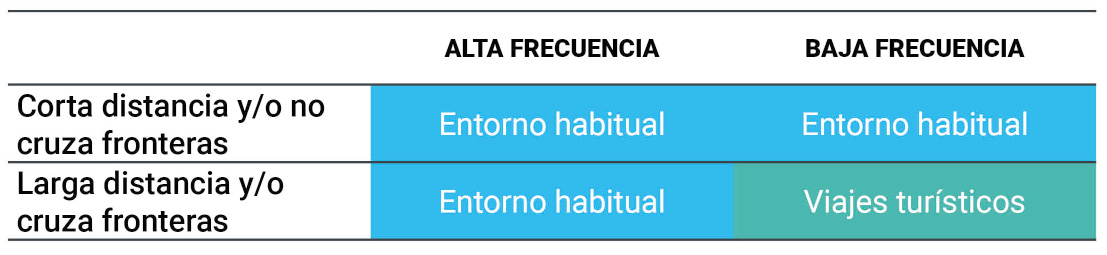
\includegraphics[width=0.8\linewidth]{imagenes/figura1.1} 

}

\caption{Entorno habitual y viajes turísticos}\label{fig:entornoYviajes}
\end{figure}

En el caso de los desplazamientos internacionales, el traspaso de las fronteras da cuenta de la dimensión de distancia mínima, sin importar la distancia recorrida\footnote{Sin embargo, un problema de particular relevancia se registra en el caso de las fronteras terrestres internacionales a partir del tránsito vecinal fronterizo (TVF), es decir, los movimientos de las personas que viven cerca de las fronteras y las cruzan con frecuencia por múltiples motivos (visitas a familiares, búsqueda de oportunidades de trabajo, compras, etc.). La medición de estos movimientos como movimientos turísticos puede tener un grave efecto distorsivo sobre las estadísticas de turismo y trae aparejadas dificultades teóricas y prácticas. La OMT recomienda, en estos casos, buscar la coordinación metodológica también con los países vecinos.}. Contrariamente, como se mencionó, a la hora de adoptar un criterio de distancia mínima relativo al turismo al interior de un país, existen posiciones diversas basadas en las particularidades de cada país, que los lleva a adoptar un radio en kilómetros, el cruce de fronteras entre unidades subnacionales o una combinación de ambas\footnote{En 2003, a pedido de la OMT, especialistas de Canadá y España relevaron los criterios de frecuencia y distancia en la definición del entorno habitual en treinta países. En ese entonces, la mayoría de los países se abstenía de utilizar un criterio claro de frecuencia; sin embargo, entre quienes lo hacían el criterio semanal era el más utilizado. En el caso de la distancia, para el cual dos tercios de los países fijaban explícitamente algún tipo de definición, el cruce de fronteras administrativas era el criterio más común, aunque en no pocos casos se utilizaba el criterio de distancia o bien una combinación entre ambos. Incluso, un país, tomaba como punto de corte una determinada cantidad de tiempo de viaje.}.

Lo expuesto deja en evidencia que la definición operacional de los criterios de distancia y frecuencia para dirimir el entorno habitual resultan cruciales para las estadísticas de turismo, ya que alteran el flujo de visitantes a contabilizar (al determinar quién es y quién no es un visitante) y, con ello, los perfiles de los visitantes, el volumen del gasto turístico, etc.

Por ejemplo, asumiendo una definición de entorno habitual que plantee una distancia mínima de 20 kilómetros y una frecuencia semanal, si una persona reside en la Ciudad de Córdoba y viaja todas las semanas a Rosario (donde realiza un estudio de posgrado), tanto la Ciudad de Córdoba como Rosario formarán parte de su entorno habitual: ningún paseo o concurrencia a un restaurante o a un espectáculo cultural que realice esta persona dentro de esas zonas será una actividad turística (incluso si se trata de lugares que nunca antes visitó). Sin embargo, si esa misma persona una vez por mes viaja hasta La Falda (distante a 60 km de la capital provincial), este desplazamiento sí constituirá un viaje turístico.~

Por otra parte, el traspaso de una frontera internacional no implica necesariamente una salida del entorno habitual ni, por tanto, un viaje turístico.~

En el caso de una persona que resida en la Ciudad Autónoma de Buenos Aires y que, por un lado viaje a Montevideo (Uruguay) todas las semanas y, que por otro lado, vaya a pescar durante medio día a Chascomús (a 120 km. de Buenos Aires) una vez cada dos o tres meses, sus viajes a Montevideo no constituirán viajes turísticos (por su alta frecuencia, que hacen que dicha ciudad~ forme parte de su entorno habitual, si bien se encuentra lejos de su lugar de residencia habitual y fuera de fronteras administrativas). En cambio, los viajes de pesca a Chascomús, con ida y vuelta en el día, sí representarán un viaje turístico, ya que implican un desplazamiento hacia fuera del entorno habitual.

El ejemplo hipotético que se presenta a continuación pone en juego dos definiciones distintas del criterio de distancia y los efectos que ello acarrearía en la medición del turismo.

En la Ciudad Verde se realiza un festival folclórico al que asisten 100 mil personas. De ellas, 20 mil son residentes en la misma ciudad (10 mil son varones y otro tanto mujeres) y gastan \$2 millones, mientras que 40 mil provienen de la Ciudad Roja (todos son varones y en conjunto gastan~ \$10 millones), ubicada a 30 kilómetros de distancia, dentro del mismo departamento. Los restantes 40 mil asistentes provienen de Ciudad~ Amarilla, ubicada en otro departamento y a 100 kilómetros, se reparten en partes iguales entre varones y mujeres y en conjunto gastan \$30 millones.

La opción 1 considera que el entorno habitual, en su dimensión geográfica, está determinado por un radio de 20 kilómetros, mientras que la opción 2 parte de asumir que sólo el traspaso de las fronteras municipales implica una salida del entorno habitual. Ahora bien, ¿qué resultados arrojarían las estadísticas de turismo en cada caso?

\begin{figure}

{\centering 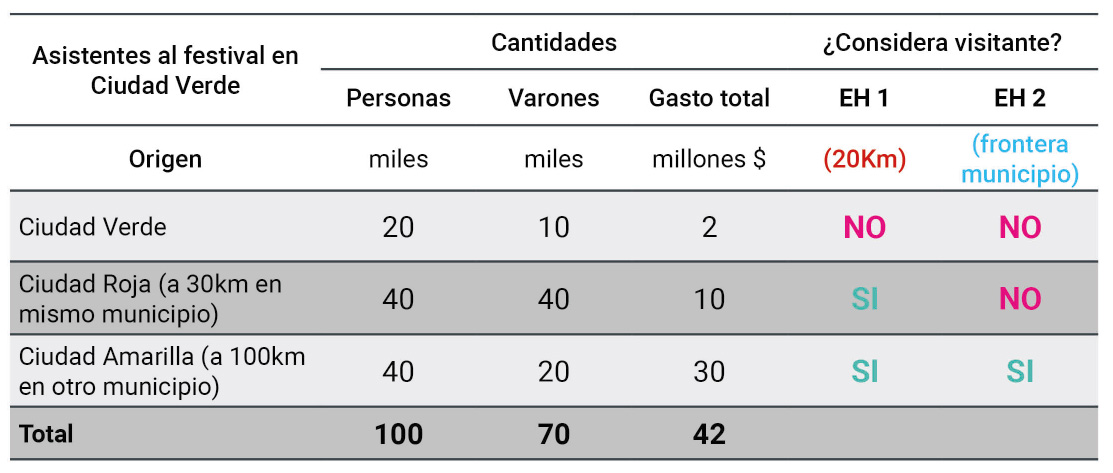
\includegraphics[width=0.8\linewidth]{imagenes/figura1.2} 

}

\caption{Ejemplo del impacto de diferentes definiciones del entorno habitual.}\label{fig:entorno}
\end{figure}

En ambos casos, los 20 mil residentes de la Ciudad Verde no se considerarán como visitantes, mientras que sí se considerarán como tales a las 40 mil personas que provienen de Ciudad Amarilla. En el caso de los residentes de la Ciudad Roja, su contabilización como visitantes dependerá de qué definición de entorno habitual se aplique.

En la opción 1, los asistentes provenientes de la Ciudad Roja serán considerados como visitantes, puesto que residen a más de 20 kilómetros de la Ciudad Verde. Entonces, en total, se contabilizarán 80 mil visitantes (de las ciudades Roja y Amarilla) que gastarán \$40 millones, a razón de \$500 por cada uno de ellos. Además, los varones representarán el 75\% de los visitantes.

En cambio, en la opción 2, los asistentes residentes en la Ciudad Roja no serán considerados visitantes puesto que entre ambas ciudades no media un traspaso de frontera municipal y, por tanto, la Ciudad Verde (donde se desarrolla el festival) forma parte del entorno habitual. Como resultado, se contabilizarán 40 mil visitantes (únicamente los residentes en Ciudad Amarilla) que gastarán \$30 millones, con un promedio \$750 por cada uno de ellos, entre los cuales el 50\% serán varones.

Como se observa, la utilización de diferentes criterios de entorno habitual conlleva resultados distintos tanto en el volumen como en la caracterización de los visitantes.

Como ya se señaló, las pautas internacionales no brindan un criterio específico para definir cuán geográficamente grande o pequeño debería ser este entorno habitual, ni cuán frecuentes la visitas a un destino para que éste pase a formar parte del entorno habitual, aunque en este último caso, tiende a imponerse el criterio de frecuencia semanal. El desafío queda entonces librado a las decisiones metodológicas de las instituciones encargadas de elaborar estadísticas del turismo.

Un ejemplo nacional de importancia es el criterio aplicado en la Encuesta de Viajes y Turismo de los Hogares (EVyTH). En este estudio el entorno habitual se operacionaliza de acuerdo a (i) el criterio de frecuencia semanal y (ii) el criterio de distancia, considerando como punto de corte dos magnitudes distintas: 40km. para los residentes en el Gran Buenos Aires y 20 km. para los residentes en los grandes aglomerados del Interior del país.

En resumen, la definición del entorno habitual de las personas constituye un problema central para la captación estadística del fenómeno turístico. Donde otras cuestiones aparecen unívocamente definidas en las recomendaciones internacionales y/o son fácilmente construibles en forma clara, precisa y comparable, el entorno habitual presenta importantes desafíos para la consolidación de un sistema nacional de estadísticas.

Debido a los efectos que trae aparejados su definición, es de absoluta relevancia que, una vez esclarecido, el entorno habitual sea operacionalizado en los instrumentos de recolección de información, y donde ello no sea posible, o lo sea en forma parcial, se debería dar precisa cuenta de las diferencias respecto al concepto original y de los posibles sesgos que se introducen.

Si el concepto de entorno habitual no es tratado adecuadamente, se correrá el riesgo de que un operativo subestime o sobreestime el impacto del turismo. En cualquier caso, no sólo no se estaría dando cuenta del impacto real del turismo sino que, en caso de contarse con dos operativos, se estaría obteniendo información no comparable.

\hypertarget{formas-de-turismo}{%
\subsection{Formas de turismo}\label{formas-de-turismo}}

\textbf{Óptica nacional}

El turismo (sean visitantes --turistas o excursionistas-, pernoctes, gasto o cualquier otra unidad considerada) se clasifica de acuerdo al \textbf{origen y el destino} de los visitantes en \textbf{formas de turismo}. En este punto, es crucial destacar que el origen del visitante remite siempre al lugar de residencia y no a la nacionalidad, sea esta natural o adquirida.

Las formas de turismo se pueden definir tanto desde el punto de vista de la clasificación del visitante, como desde la óptica de la unidad económica receptora. Habitualmente, se suele considerar al país como unidad económica, nivel al cual corresponden las siguientes formas de turismo:

\begin{itemize}
\item
  \textbf{Turismo interno:} visitantes que se desplazan dentro del mismo país en el que residen.
\item
  \textbf{Turismo receptivo:} visitantes no residentes que viajan al país de referencia.
\item
  \textbf{Turismo emisivo:} visitantes residentes en el país de referencia que viajan a otro país.
\end{itemize}

\begin{figure}

{\centering 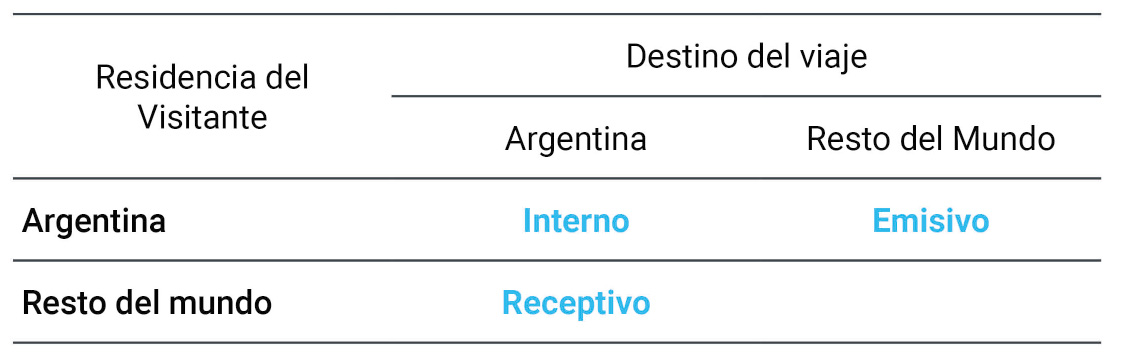
\includegraphics[width=0.8\linewidth]{imagenes/figura1.3} 

}

\caption{Formas de turismo desde la óptica nacional}\label{fig:nacional}
\end{figure}

La combinación de pares de estos tipos de turismo da lugar a otros tres subconjuntos:

\begin{itemize}
\item
  \textbf{Turismo Interior:} Interno + Receptivo.
\item
  \textbf{Turismo Nacional:} Interno + Emisivo.
\item
  \textbf{Turismo Internacional:} Emisivo + Receptivo.
\end{itemize}

Esta clasificación parte de considerar como unidad mínima al nivel nacional, pero su lógica puede aplicarse, como se verá más adelante, a una provincia u otro nivel administrativo menor.

\hypertarget{uxf3ptica-provincial}{%
\section{Óptica provincial}\label{uxf3ptica-provincial}}

\textbf{Complejidad de la medición del turismo desde una óptica provincial}

La contabilización de los visitantes que viajan desde o hacia una unidad económica de referencia (sea ésta nacional, provincial o municipal)\footnote{Estas unidades suelen ser económicas y políticas a la vez: país, provincia, municipio o departamento, ciudad o localidad.} presenta dos tipos de dificultades.

La primera está constituida por los \textbf{problemas de captación} o medición de los visitantes y se relaciona con las propias características de los viajes turísticos: algunos de ellos son de mayor facilidad de medición que otros.

El segundo grupo de dificultades refiere a los inconvenientes para contabilizar correctamente a los visitantes en unidades menores cuando un viaje turístico incluye dos o más paradas o visitas, y podrían denominarse \textbf{problemas de agregación:} cuanto menor es el tamaño geográfico de la unidad económica de referencia, mayor es la complejidad de alcance.

Lógicamente, presentarlas por separado no implica que no existan diversos entrecruzamientos entre ambos tipos de dificultades.

\hypertarget{problemas-de-captaciuxf3n}{%
\subsection{Problemas de captación}\label{problemas-de-captaciuxf3n}}

Cómo se mencionó, las dificultades de captación obedecen a las características del viaje emprendido por el visitante. Independientemente de la existencia de operativos estadísticos de medición o de la potencial posibilidad de realizarlos, las características que asuma el viaje de cada visitante determinan mayores o menores dificultades para su abordaje.~

Un inconveniente adicional, y anterior, a este tipo de problemas, está dado por la confusión que puede existir entre el turismo como categoría o concepto técnico o metodológico y el turismo como categoría nativa o de sentido común: muchas personas pueden interpretar que hacen turismo sólo cuando realizan desplazamientos por motivos de vacaciones, recreo o esparcimiento y por una cantidad elevada de días. Sin embargo, como se ha visto en el capítulo anterior, se considera turismo a la actividad de todos los visitantes durante sus viajes turísticos, esto es, de las salidas de su entorno habitual, independientemente de cuál sea el motivo (vacaciones o recreación, pero también visita a familiares o amigos, negocios, estudios, compras, trámites, peregrinaciones, etc.) o la extensión del viaje\footnote{Lógicamente, de acuerdo a lo expuesto anteriormente, no se consideran viajes turísticos aquellos viajes en los que la finalidad principal haya sido ser empleado por una unidad económica del lugar de destino, así que tampoco aquellos desplazamientos con una duración superior al año.

  \hfill\break
}.~

Por citar un ejemplo extremo, desde el marco metodológico de la estadística de turismo, es tan visitante un australiano que se queda en las Cataratas del Iguazú durante un mes como un residente en Posadas que visita en el día a un pariente lejano que reside en L. N. Alem, ciudad del interior de la provincia de Misiones distante a 75 km. de la capital.

Esta cuestión tiene varias aristas. En primer lugar, cuando se realizan operativos estadísticos basados en encuestas, se debe \textbf{evitar mencionar la palabra turismo} para no generar confusiones en los entrevistados.

Por ejemplo, una persona que residió en una ciudad hace años y vuelve allí con cierta asiduidad a visitar a sus familiares, probablemente no se considere a sí mismo turista, aunque obviamente debe englobarse dentro del concepto técnico.~

Una posible solución para evitar este inconveniente es mencionar la palabra \textbf{viaje}, que para el común de la gente tiene un sentido más amplio que turismo, y, a continuación, hacer referencia a ejemplos de los múltiples motivos que pueden originar un viaje turístico.

En segundo lugar, y con mayor efecto aún sobre los resultados, es necesario que los propios responsables de la producción o compilación de estadística de turismo sean absolutamente conscientes de la amplitud del concepto de turismo, procurando dar cuenta de la totalidad del fenómeno. Usualmente, esto no resulta posible por diversas razones (técnicas, económicas, etc.), pero es preciso tener presente y hacer explícito qué parte del fenómeno turístico miden y qué parte no miden los operativos estadísticos existentes.

Aún cuando lo anterior sea claro, no todos los viajes turísticos son capturables desde el punto de vista estadístico con el mismo nivel de esfuerzo, derivando en la necesidad de priorizar la medición de ciertos segmentos (por ejemplo, los turistas que se alojan en hoteles). Nuevamente, lo importante aquí es tener presente qué es lo que queda por fuera del recorte que el/los operativo/s de medición vigentes proponen\footnote{Al respecto, una estrategia relativamente sencilla de estimar el flujo total de turismo interior podría surgir de un correcto seguimiento a un segmento, a partir del cual realizar una proyección al total. Por ejemplo, mediante una encuesta continua de ocupación de alojamientos hoteleros y parahoteleros es posible estimar el subuniverso de los turistas que allí se alojan. Por otra parte, realizar una encuesta de caracterización de perfil del turista (demanda) cada una determinada cantidad de años (3 o 5, por ejemplo, o también todos los años) permitiría conocer qué participación tiene el segmento medido sobre el total y a partir de ello estimar el volumen total de turistas.}.

Por ejemplo, si la localidad A recibe en un año 1.000 turistas que se alojan en hoteles y mediante una encuesta de perfil del turista se determina que quienes se alojan en hoteles representan el 25\% del total de turistas que visitan esa localidad, mediante una ``regla de tres'' se puede estimar el volumen total de turistas: \(1.000\) * \(100\%\) / \(25\%\) = \(4.000\).

Este ejemplo estilizado no debe hacer perder de vista que una estimación de este tipo se podrá realizar siempre y cuando se cumplan determinados requisitos metodológicos y técnicos, de modo tal que se pueda garantizar tanto que la encuesta de caracterización de la demanda refleje ``realmente'' la estructura de segmentos que componen el universo del turismo interior, lo cual no es nada sencillo, como que la medición de los turistas alojados en hoteles sea robusta y confiable.

Además de las encuestas de ocupación de alojamientos y de las encuestas de caracterización de la demanda, los registros administrativos (vehículos en peajes, entradas vendidas para atractivos del destino, consultas en centros de información turística, etc.) constituyen una excelente fuente para realizar estimaciones de este tipo (por su robustez y, en general, bajo o nulo costo), siempre y cuando, nuevamente, reciban el tratamiento metodológico adecuado.

La Figura \ref{fig:dificultad} presenta, de modo estilizado, aquellas características que, en las distintas dimensiones del viaje, suponen diferentes niveles de dificultad para la captación de los visitantes\footnote{Estas apreciaciones no tratan sobre una cuestión marginal: según los datos de la EVyTH sobre turismo interno del año 2012, tres de cada cinco turistas se alojaron en viviendas de familiares o amigos o en segundas viviendas del hogar, dos de cada cinco turistas no viajaron por ocio y dos tercios de los turistas se desplazaron en un automóvil particular.}.

\begin{figure}

{\centering 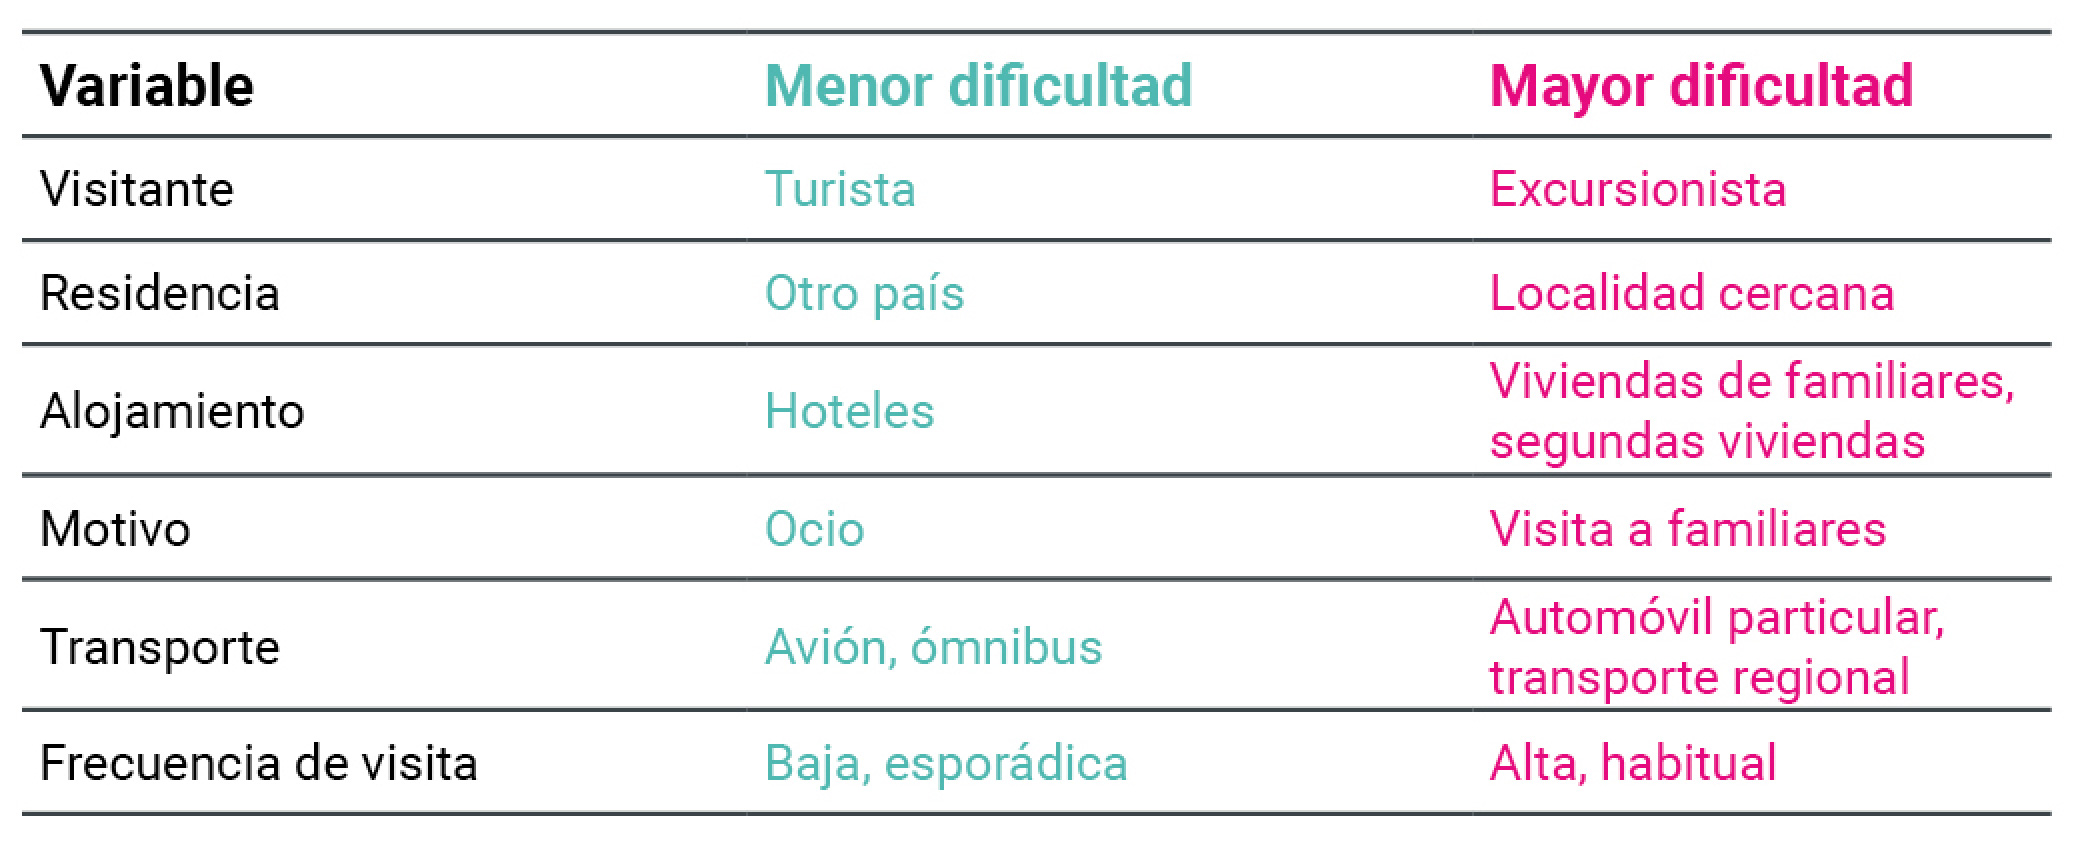
\includegraphics[width=0.8\linewidth]{imagenes/figura1.4} 

}

\caption{Nivel de dificultad en la captación según características del viaje turístico.}\label{fig:dificultad}
\end{figure}

Cabe señalar que el sesgo que estos problemas introducen es menor en encuestas a hogares o cuando se logra entrevistar al visitante al final de su viaje (en puntos de salida del destino, por ejemplo) que en las encuestas que se realizan en el/los destino/s visitado/s\footnote{Una encuesta realizada en el lugar de residencia podrá captar todos los viajes que los entrevistados realizaron, del mismo modo que una encuesta cuya cobertura alcance a todos los puntos de salida de un destino (por distintas vías) permitirá encuestar a todos los visitantes independientemente de las características de su viaje. En cambio, si las encuestas se realizan en lugares de ``interés turístico'' (sitios, calles, etc.) del destino, probablemente se subestime la captación de ciertos segmentos que no realizan actividades típicamente turísticas (por ejemplo, quien viaja a visitar familiares), mientras que ese problema no estaría presente (o al menos no en la misma magnitud) entre quienes se alojan en hoteles, visitan los puntos típicos, etc.}.

Cómo se analizó en el capítulo anterior, la definición del entorno habitual y las discusiones que apareja también pueden englobarse dentro de este grupo de complejidades, puesto que si cada provincia toma una decisión operacional sin considerar al resto, los resultados obtenidos no serán estrictamente comparables. En consecuencia, esto implica necesariamente, para evitar tal situación, que cada uno de los criterios adoptados por las provincias deberían partir de los mismos principios ordenadores, aún cuando sea posible (y hasta necesario) que los criterios~ difieran entre sí en algún elemento específico (por caso, no implica lo mismo 20km. en provincias pequeñas y densamente pobladas como Misiones o Tucumán que en provincias extensas y escasamente pobladas como Chubut o Santa Cruz).

\hypertarget{problemas-de-agregaciuxf3n-visitantes-y-llegadas-de-visitantes}{%
\subsection{Problemas de agregación: visitantes y llegadas de visitantes}\label{problemas-de-agregaciuxf3n-visitantes-y-llegadas-de-visitantes}}

En este caso, las complejidades se presentan cuando se procura medir el turismo en unidades geográficas de carácter subnacional (provincias, departamentos/partidos, municipios o localidades en el caso argentino), y se relacionan con la clasificación y contabilización de los visitantes.

Cabe señalar que, además de las razones lógicas (es más sencillo contabilizar ingresos o egresos de un país que de una provincia o ciudad, por ejemplo), en alguna medida, este tipo de inconveniente se relaciona con el enfoque internacional de las estadísticas de turismo, donde las prescripciones metodológicas suelen centrarse en las entidades nacionales y donde sólo recientemente ha comenzado a prestarse atención a las estimaciones desde niveles subnacionales.

Sin dudas, cuando se hace referencia a las dificultades de agregación el principal problema está dado por la contabilización de los visitantes que incluyen en sus viajes dos o más paradas o visitas turísticas, que, en la óptica de medición desde el destino, pueden denominarse \textbf{llegadas de visitantes}.

Por definición, la cantidad de visitantes a una provincia siempre será igual o menor a la cantidad de llegadas de visitantes a las localidades que la componen. Si todas las ciudades de una provincia sumarán los turistas que las visitaron (y pernoctaron en ellas), el número de llegadas a las localidades provinciales sería mayor al número de turistas (es decir, personas que realizaron viajes fuera de su entorno habitual), salvo en el caso extremo de que todos los visitantes hayan visitado un solo lugar durante su viaje turístico.

Esto mismo aplica a la medición del turismo en un país a partir del agregado de los datos provinciales. Incluso, siguiendo con esta lógica, sucede con la cantidad de visitantes a nivel mundial respecto a la suma de llegadas de visitantes de los países.

Cabe señalar que los operativos estadísticos que consideran la oferta de servicios turísticos o bien que contabilizan a los visitantes que arriban a una unidad de referencia (provincia, ciudad, etc.) en la propia unidad, no cuentan visitantes en sentido estricto sino llegadas de visitantes\footnote{La contabilización ``perfecta'' de visitantes podría realizarse únicamente a partir de encuestas a hogares (entrevistando a los visitantes una vez finalizado el viaje) o de encuestas en destinos que garanticen la no duplicación (como el caso de la Encuesta de Turismo Internacional, que encuesta a las personas al momento de la finalización de su viaje). Obviando las implicancias de la definición de destino adoptada (provincia, ciudad, etc.), si se relevase la totalidad de destinos visitados a lo largo del viaje, a partir de este tipo de operativos podría estimarse tanto la cantidad de visitantes como la de llegadas de visitantes.}.

Una vez más queda en evidencia el lugar central que ocupa la metodología en la medición del turismo: a diferencia del visitante (excursionista o turista), el concepto de llegada de visitante carece de una definición unívoca, aún cuando juega un rol crucial en la estadística subnacional, creciendo en su importancia a medida que disminuye el tamaño de la unidad de referencia considerada.

El concepto de llegada de visitantes está íntimamente relacionado a la consideración de un \textbf{destino} en la metodología de cada operativo de medición.~

\hfill\break

Así, sí el corte se considera a nivel provincial, un visitante que tuvo paradas turísticas en tres ciudades de dos provincias diferentes será contabilizado dos veces (una en cada provincia). En cambio, si se considera como destino cada ciudad o localidad, la cantidad de llegadas de visitantes que se registrarán en ese caso serán tres (dos en una de las provincias y una en la otra).

Aún restaría definir, más allá del alcance geográfico, qué requisitos se deberían cumplir para que el arribo de un visitante se considere una visita o parada turística o, lo que es lo mismo, una llegada de visitante. En este punto, vale recordar que las recomendaciones internacionales establecen una duración mínima y/o la realización de algún tipo de consumo.~

Por esta misma razón, un turista (una persona que se desplaza fuera de su entorno habitual por al menos una noche), desde la óptica del destino puede ser contabilizado como excursionista si realiza allí una visita turística sin pernocte.

Por ejemplo, si una ciudad contabiliza como llegadas de visitantes a todos aquellos visitantes que se detienen a apreciar un atractivo natural del lugar, aunque sea por pocos minutos, mientras que otra ciudad cercana sólo cuenta a aquellos visitantes que pasan al menos dos horas en ella, los datos provenientes de uno y otro caso no podrán ser comparados en forma directa. Puede que, en este caso, la comparabilidad de los datos no sea relevante para ambas ciudades,~ por lo que no considerarán necesario aunar criterios, puesto que la definición que cada una de ellas ha considerado sirve mejor a sus propósitos. Sin embargo, sí sería un error metodológico que desde el nivel provincial se pretenda estimar el volumen de llegadas de visitantes a localidades simplemente añadiendo la información que provee cada una de las localidades. Mayor sería aún el error si se pretende asimilar que la suma de la información brindada por estas ciudades expresa la cantidad de visitantes, puesto que no sólo se estaría cometiendo el error de sumar llegadas de visitantes definidas de modo diferente (y que, por tanto, dan cuenta de cosas distintas), sino que también se estaría incurriendo en posibles sobreestimaciones al contabilizar dos veces a un mismo visitante que estuvo en ambas localidades.

Sin dudas, las limitaciones siempre existen y resulta harto complejo, sino imposible, cumplir de manera absoluta con todos los principios y cuidados metodológicos. No obstante, nuevamente, resulta imprescindible que los equipos técnicos de producción de estadística de turismo, ya sean a nivel nacional, provincial o local, sean plenamente conscientes de cuál es la verdadera unidad de la cual la metodología utilizada en una operación estadística determinada da cuenta, para no caer en confusiones, errores o sesgar los resultados, o, si no hay más remedio que caer en ellos, para poder analizar la información obtenida con los reparos necesarios.

El ejemplo siguiente ayuda a comprender mejor los puntos aquí tratados.

Una persona inicia un viaje turístico el 10 de enero y lo finaliza el 20 de enero, visitando y pernoctando en hoteles de dos localidades (3 noches en una y 7 noches en otra) de una misma provincia. De acuerdo al tipo de operativo, la contabilización de este visitante será diferente.

\begin{figure}

{\centering 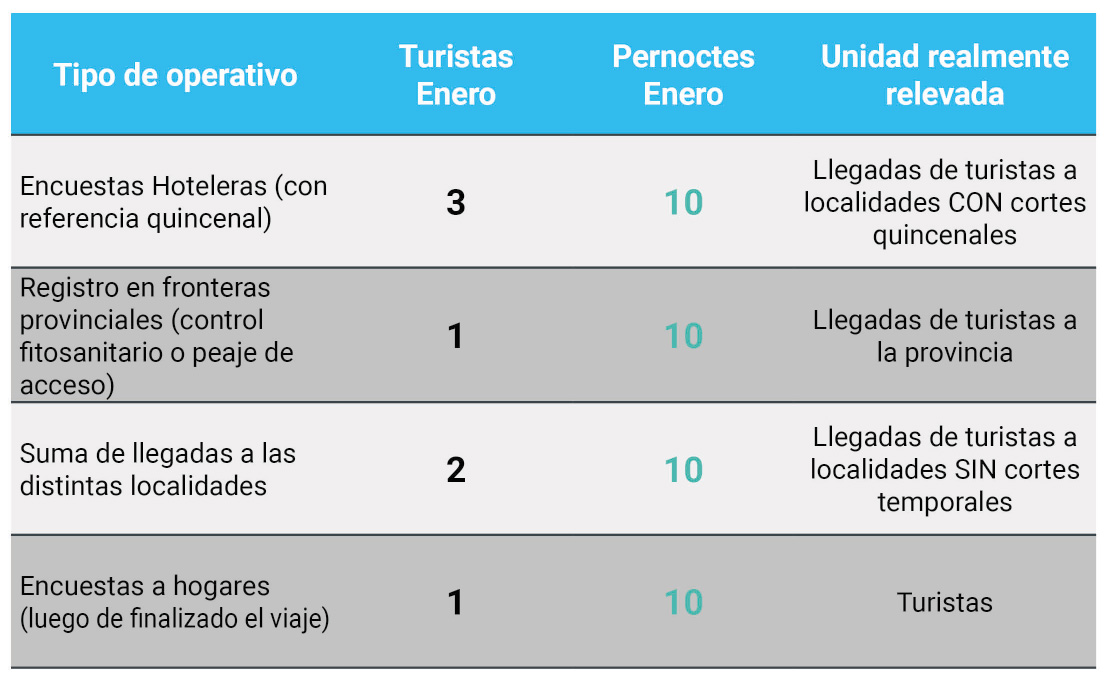
\includegraphics[width=0.8\linewidth]{imagenes/figura1.5} 

}

\caption{Ejemplo de diferentes resultados a partir de distintos operativos estadísticos}\label{fig:operativos}
\end{figure}

Sin considerar otras múltiples aristas que deberían intervenir y complejizar la discusión, este sencillo ejemplo demuestra cómo diferentes operativos, con sus respectivas metodologías e instrumentos, contabilizarían un mismo fenómeno de manera distinta.

Otro dato a resaltar, como puede observarse en este ejemplo, es que, para el caso de los turistas y cuando se utilicen modelos de obtención de resultados a partir del compendio de estadística local, \textbf{la adición de los pernoctes no está atravesada por los problemas de duplicación y, por tanto, constituyen un indicador más robusto.}

\hypertarget{formas-de-turismo-desde-la-uxf3ptica-provincial}{%
\subsection{Formas de turismo desde la óptica provincial}\label{formas-de-turismo-desde-la-uxf3ptica-provincial}}

Lo expuesto permite deducir que, desde una óptica subnacional, es preciso contemplar una manera más ajustada de clasificar las formas de turismo.

La clasificación de la OMT parte de considerar como unidad mínima al nivel nacional, pero su lógica puede aplicarse a una provincia u otro nivel administrativo menor.

De este modo, tomando como referencia a una provincia, pueden identificarse cinco formas básicas de turismo, tal como se observa en la Figura \ref{fig:formasturismo}

\begin{figure}

{\centering 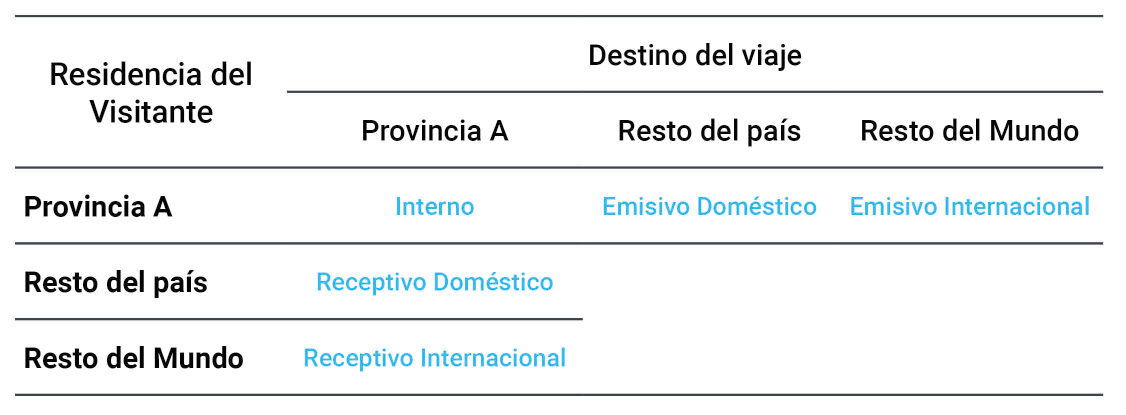
\includegraphics[width=0.8\linewidth]{imagenes/figura1.6} 

}

\caption{Formas de turismo desde la óptica provincial}\label{fig:formasturismo}
\end{figure}

De la combinación de las formas expuestas precedentemente se desprenden otras categorías:

\begin{itemize}
\item
  \textbf{Provincial Doméstico}: Interno + Emisivo doméstico.
\item
  \textbf{Provincial Total}: Interno + Emisivo doméstico + Emisivo Internacional.
\item
  \textbf{Interior Doméstico}: Interno + Receptivo Doméstico.
\item
  \textbf{Interior Total}: Interno + Receptivo Doméstico + Receptivo Internacional.
\end{itemize}

\hypertarget{la-experiencia-internacional}{%
\subsection{La experiencia internacional}\label{la-experiencia-internacional}}

\textbf{Medición del turismo desde unidades económicas subnacionales}

Llegado este punto, es interesante conocer cómo algunos países han logrado obtener estimaciones para el flujo turístico total en entidades subnacionales.

En primer lugar, cabe mencionar que pocos son los países que logran obtener realmente este tipo de resultados y cuando se presenta algún resultado que pretende dar cuenta de este tópico, un análisis detallado indica que sólo se refleja parcialmente el universo posible de visitantes, con un marcado sesgo hacia el turismo internacional.

A nivel mundial, los países con mayor desarrollo de sus sistemas de estadística de turismo (y de sus sistemas estadísticos en general), son aquellos que logran realizar estimaciones como las planteadas.

Dos casos paradigmáticos son los de España y Canadá, ambos con una amplia y sólida trayectoria en la medición del turismo.

\textbf{España} cuenta con una encuesta de turismo nacional, relevada en hogares (Encuesta de turismo de residentes -ETR/FAMILITUR-) que permite conocer el origen y destino de todos los viajes turísticos que realizan los residentes de ese país. Esta encuesta cuenta con representatividad a nivel de comunidad autónoma (el equivalente a las provincias en Argentina) e incluye en su cobertura a toda la población, independientemente del contexto (rural, urbano) en que resida.

Por otra parte, posee un relevamiento de movimientos fronterizos a partir del cual da cuenta del turismo internacional (FRONTUR), mientras que a partir de una encuesta de caracterización y gasto del turismo internacional (EGATUR), que incluye todos sus segmentos (al contemplar la totalidad de las vías de acceso en su muestra) puede estimar cuanto de este flujo corresponde a cada comunidad autónoma.

En este marco, las comunidades autónomas pueden realizan sus estimaciones de visitantes (fundamentalmente turistas), tanto para la emisión como para la recepción, a partir de los datos que surgen de los operativos nacionales cuya cobertura y robustez es suficiente para ello.\\
ETR/FAMILITUR constituye el insumo fundamental para captar los viajes realizados por los residentes dentro del país (turismo interno a nivel nacional, turismo interno y turismo receptivo y emisivo doméstico desde la mirada provincial), en tanto que FRONTUR y EGATUR son utilizadas para dimensionar la relevancia del turismo (receptivo y emisivo) internacional para cada comunidad autónoma.

Además, las encuestas nacionales de ocupación de alojamientos turísticos (que relevan no sólo el sector hotelero y parahotelero, sino también los campings y los departamentos de alquiler turístico), también con representatividad por comunidad autónoma, permiten la desagregación del turismo al interior de cada comunidad de acuerdo a esta variable.

Cabe señalar que la cuantificación de pernoctaciones, de acuerdo a lo observado en las publicaciones, adquiere igual o mayor relevancia que la cuantificación de visitantes.\\
Una limitación de los operativos españoles es que relevan, tanto ETR/FAMILITUR como EGATUR, el destino principal del viaje, lo que implica que un visitante que ha recorrido más de una comunidad autónoma durante su viaje será contabilizado solo en una de ellas.

Finalmente, en los apartados metodológicos de los estudios publicados no se precisa~ qué sucede con la consistencia entre información brindada por diferentes fuentes (por ejemplo, la cantidad de residentes que viajan al exterior captados por ETR/FAMILITUR y por FRONTUR/EGATUR, o bien los pernoctes que surgen de las encuestas de ocupación de alojamientos y los pernoctes que surgen de encuestas realizadas a los visitantes).

Links:

\href{https://www.ine.es/dyngs/INEbase/es/operacion.htmc=Estadistica_C\&cid=1254736176990\&menu=ultiDatos\&idp=1254735576863}{ETR/Familitur Encuesta de turismo de residentes}

\href{https://www.ine.es/dyngs/INEbase/es/operacion.htmc=Estadistica_C\&cid=1254736176996\&menu=ultiDatos\&idp=1254735576863}{FRONTUR}

\href{https://www.ine.es/dyngs/INEbase/es/operacion.htmc=Estadistica_C\&cid=1254736177002\&menu=ultiDatos\&idp=1254735576863}{EGATUR}

En el caso de \textbf{Canadá}, también cuenta con una encuesta a hogares que mide el turismo nacional (National Travel Survey -NTS-) y con una encuesta de turismo internacional (Visitor Travel Survey -VTS-). En ambos casos, (y también en el de los relevamientos de ocupación de alojamientos turísticos), se trata de estudios con representatividad provincial.

A diferencia del caso español, ambas encuestas indagan no sólo por el destino principal del viaje sino por todos los destinos visitados (ciudad o localidad).

Debido a esta forma de indagación por el destino, plantea tres unidades principales.

- Personas-viajes (``persons-trips'' o ``travels''), que son los visitantes.

- Personas-visitas (``persons visits''), que equivalen a llegadas de visitantes (independientemente si pernoctan o no en destino).

- Personas visitas de al menos una noche (``visit-nights''), que pueden traducirse como llegadas de turistas.

Esta clasificación permite la reconstrucción del flujo turístico por forma de turismo para cada provincia, cuya suma, lógicamente, es superior al total nacional (y lo mismo sucede al considerar la suma de las llegadas a localidades de una provincia respecto al total de llegadas a esa provincia).

En base a lo expuesto, este modelo puede denominarse ``\textbf{aguas abajo"}, dado que se realizan estimaciones subnacionales a partir de estudios nacionales, en contraste con un modelo''\textbf{aguas arriba"}, donde los flujos turísticos nacionales son reconstruidos a partir de los datos que aportan las entidades subnacionales.

Como se verá en el Capítulo 2, Argentina cuenta hoy con este tipo de operativos nacionales necesarios para dar cuenta del flujo turístico. No obstante, estos estudios no cuentan con representatividad a niveles provinciales.

Links:

\href{https://www150.statcan.gc.ca/n1/en/subjects/travel_and_tourism}{Canadá}

\href{https://www23.statcan.gc.ca/imdb/p2SV.pl?Function=getSurvey\&SDDS=5232}{National Travel Survey (NTS)}

\href{https://www23.statcan.gc.ca/imdb/p2SV.pl?Function=getSurvey\&SDDS=5261}{Visitor Travel Survey (VTS)}

\hypertarget{encuestas-nacionales}{%
\chapter{\texorpdfstring{\textbf{Encuestas Nacionales}}{Encuestas Nacionales}}\label{encuestas-nacionales}}

\textbf{Características y Alcance}

Actualmente, el Ministerio de Turismo y Deportes de la Nación (MINTURDEP) cuenta con tres encuestas que le permiten mensurar y caracterizar el turismo, tanto a nivel nacional como a nivel regional\footnote{Las regiones turísticas definidas en sus operativos estadísticos son las siguientes: Ciudad de Buenos Aires, Provincia de Buenos Aires, Córdoba, Litoral (Corrientes, Chaco, Entre Ríos, Formosa, Misiones y Santa Fe), Norte (Catamarca, Jujuy, Salta, Santiago Del Estero, Tucumán y La Rioja), Cuyo (Mendoza, San Juan, San Luis) y Patagonia (Chubut, La Pampa, Neuquén, Río Negro, Santa Cruz y Tierra Del Fuego).}.Estos estudios son la Encuesta de Viajes y Turismo de los Hogares (\textbf{EVyTH}), la Encuesta de Ocupación Hotelera (\textbf{EOH}) y la Encuesta de Turismo Internacional (\textbf{ETI}).

En este capítulo se presentan las principales características metodológicas y las limitaciones que presentan cada una de ellas, tanto en general como para su utilización a niveles provinciales.

No obstante, cabe adelantar aquí que tanto la óptica de análisis como la cobertura de estos operativos difiere.

En cuanto a la óptica, la EVyTH y la ETI son encuestas de demanda, realizadas a los visitantes luego de finalizado su viaje (EVyTH) o al momento de finalización (ETI), mientras que la EOH es una encuesta realizada desde la perspectiva de la oferta, relevada en establecimientos hoteleros y para-hoteleros.

En relación a la cobertura, si bien algunas formas de turismo coinciden, debe tenerse presente que los universos a los que refieren son distintos.
Por ejemplo, el turismo interno (desde la óptica provincial) relevado por la EVyTH contempla los viajes de los residentes en los grandes aglomerados de una provincia a cualquier destino dentro de esa provincia; en cambio, el turismo interno que contempla la EOH cuenta los viajeros que residen en cualquier lugar de la provincia que arriban a las localidades de la provincia incluidas en su muestra.

\hypertarget{evyth}{%
\section{EVyTH}\label{evyth}}

La \textbf{Encuesta de Viajes y Turismo de los Hogares (EVyTH)} es un operativo realizado por el MINTURDEP, cuyo objetivo principal es proporcionar información sobre los viajes turísticos de los residentes de Argentina hacia dentro y fuera del país: cuándo viajan, a dónde van, qué medios de transporte utilizan, dónde se alojan, cuáles son los motivos por los que viajan, cómo organizan sus viajes, qué actividades turísticas realizan, cuánto gastan, etc.

Se trata de una encuesta realizada en forma telefónica a hogares, en la que se indaga por los viajes realizados por todas las personas que componen el hogar a lugares ubicados fuera de su entorno habitual.
El primer relevamiento se desarrolló durante todo el año 2006; el segundo tuvo lugar durante el primer trimestre de 2011; y finalmente, a partir de enero de 2012, la encuesta se realiza en forma continua.

La muestra abarca a hogares residentes en los ``grandes aglomerados urbanos'' definidos en la Encuesta Permanente a Hogares del INDEC (63\%\footnote{El Área Metropolitana de Buenos Aires (AMBA), conformada por la Ciudad de Buenos Aires y los Partidos del Gran Buenos Aires, tiene una cobertura del 100\%, mientras que en el conjunto del Interior del país la cobertura es de aproximadamente el 44\%.} del total de la población argentina, aproximadamente), excluyendo de este modo a los residentes en ciudades medianas y pequeñas, en pueblos y en zonas rurales.

Lógicamente, aquellos visitantes residentes en el exterior del país tampoco son alcanzados por este operativo.
Debido a que la encuesta se realiza en el lugar de residencia u origen de los visitantes y dada la cobertura geográfica del operativo, el análisis por origen de los visitantes estará limitado a los visitantes que provienen de los grandes aglomerados urbanos del país.
En cambio, el análisis de los resultados por destino contemplará a todas las ciudades o localidades del país.

La EVyTH indaga por el destino principal del viaje (donde pasó más noches) a nivel de ciudad o localidad.
Si el viaje incluyó alojamiento con pernocte en otras localidades además de la principal, las mismas no son identificadas, aunque sí es posible conocer la cantidad de otras localidades donde se pernoctó.

El diseño muestral de la EVyTH es probabilístico, y se encuadra en un diseño estratificado con selección sistemática al azar dentro de cada uno de los estratos.
Los estratos están conformados por las regiones turísticas utilizadas habitualmente por el MINTURDEP (con la salvedad de que se consideran dos subregiones en el caso de la Provincia de Buenos Aires: los Partidos del Gran Buenos Aires y el Interior de la Provincia de Buenos Aires).

Los resultados de la EVyTH se presentan con períodos de referencia trimestrales.
Los mismos surgen de la agregación de datos calculados a nivel mensual en muestras independientes.
A nivel nacional, las estimaciones mensuales se realizan sobre una muestra de alrededor de 5.200 hogares, integrados por unas 16 mil personas.

Debido a que la encuesta fue diseñada para obtener resultados a niveles regionales, las estimaciones provinciales deben ser consideradas con cautela dado que la cantidad de hogares encuestados en los aglomerados de cada provincia varía sustancialmente.
Llógicamente, a mayor cantidad de muestra, las estimaciones presentarán mayor fiabilidad (menor error estadístico, véase Figura 2.1).

\textbf{Figura 2.1. Cantidad aproximada de casos muestrales (hogares) sobre las que se realizan las estimaciones mensuales y participación de él o los grandes aglomerados urbanos (GAU) considerados por la EVyTH sobre el total de la población de cada provincia.}

\begin{figure}

{\centering 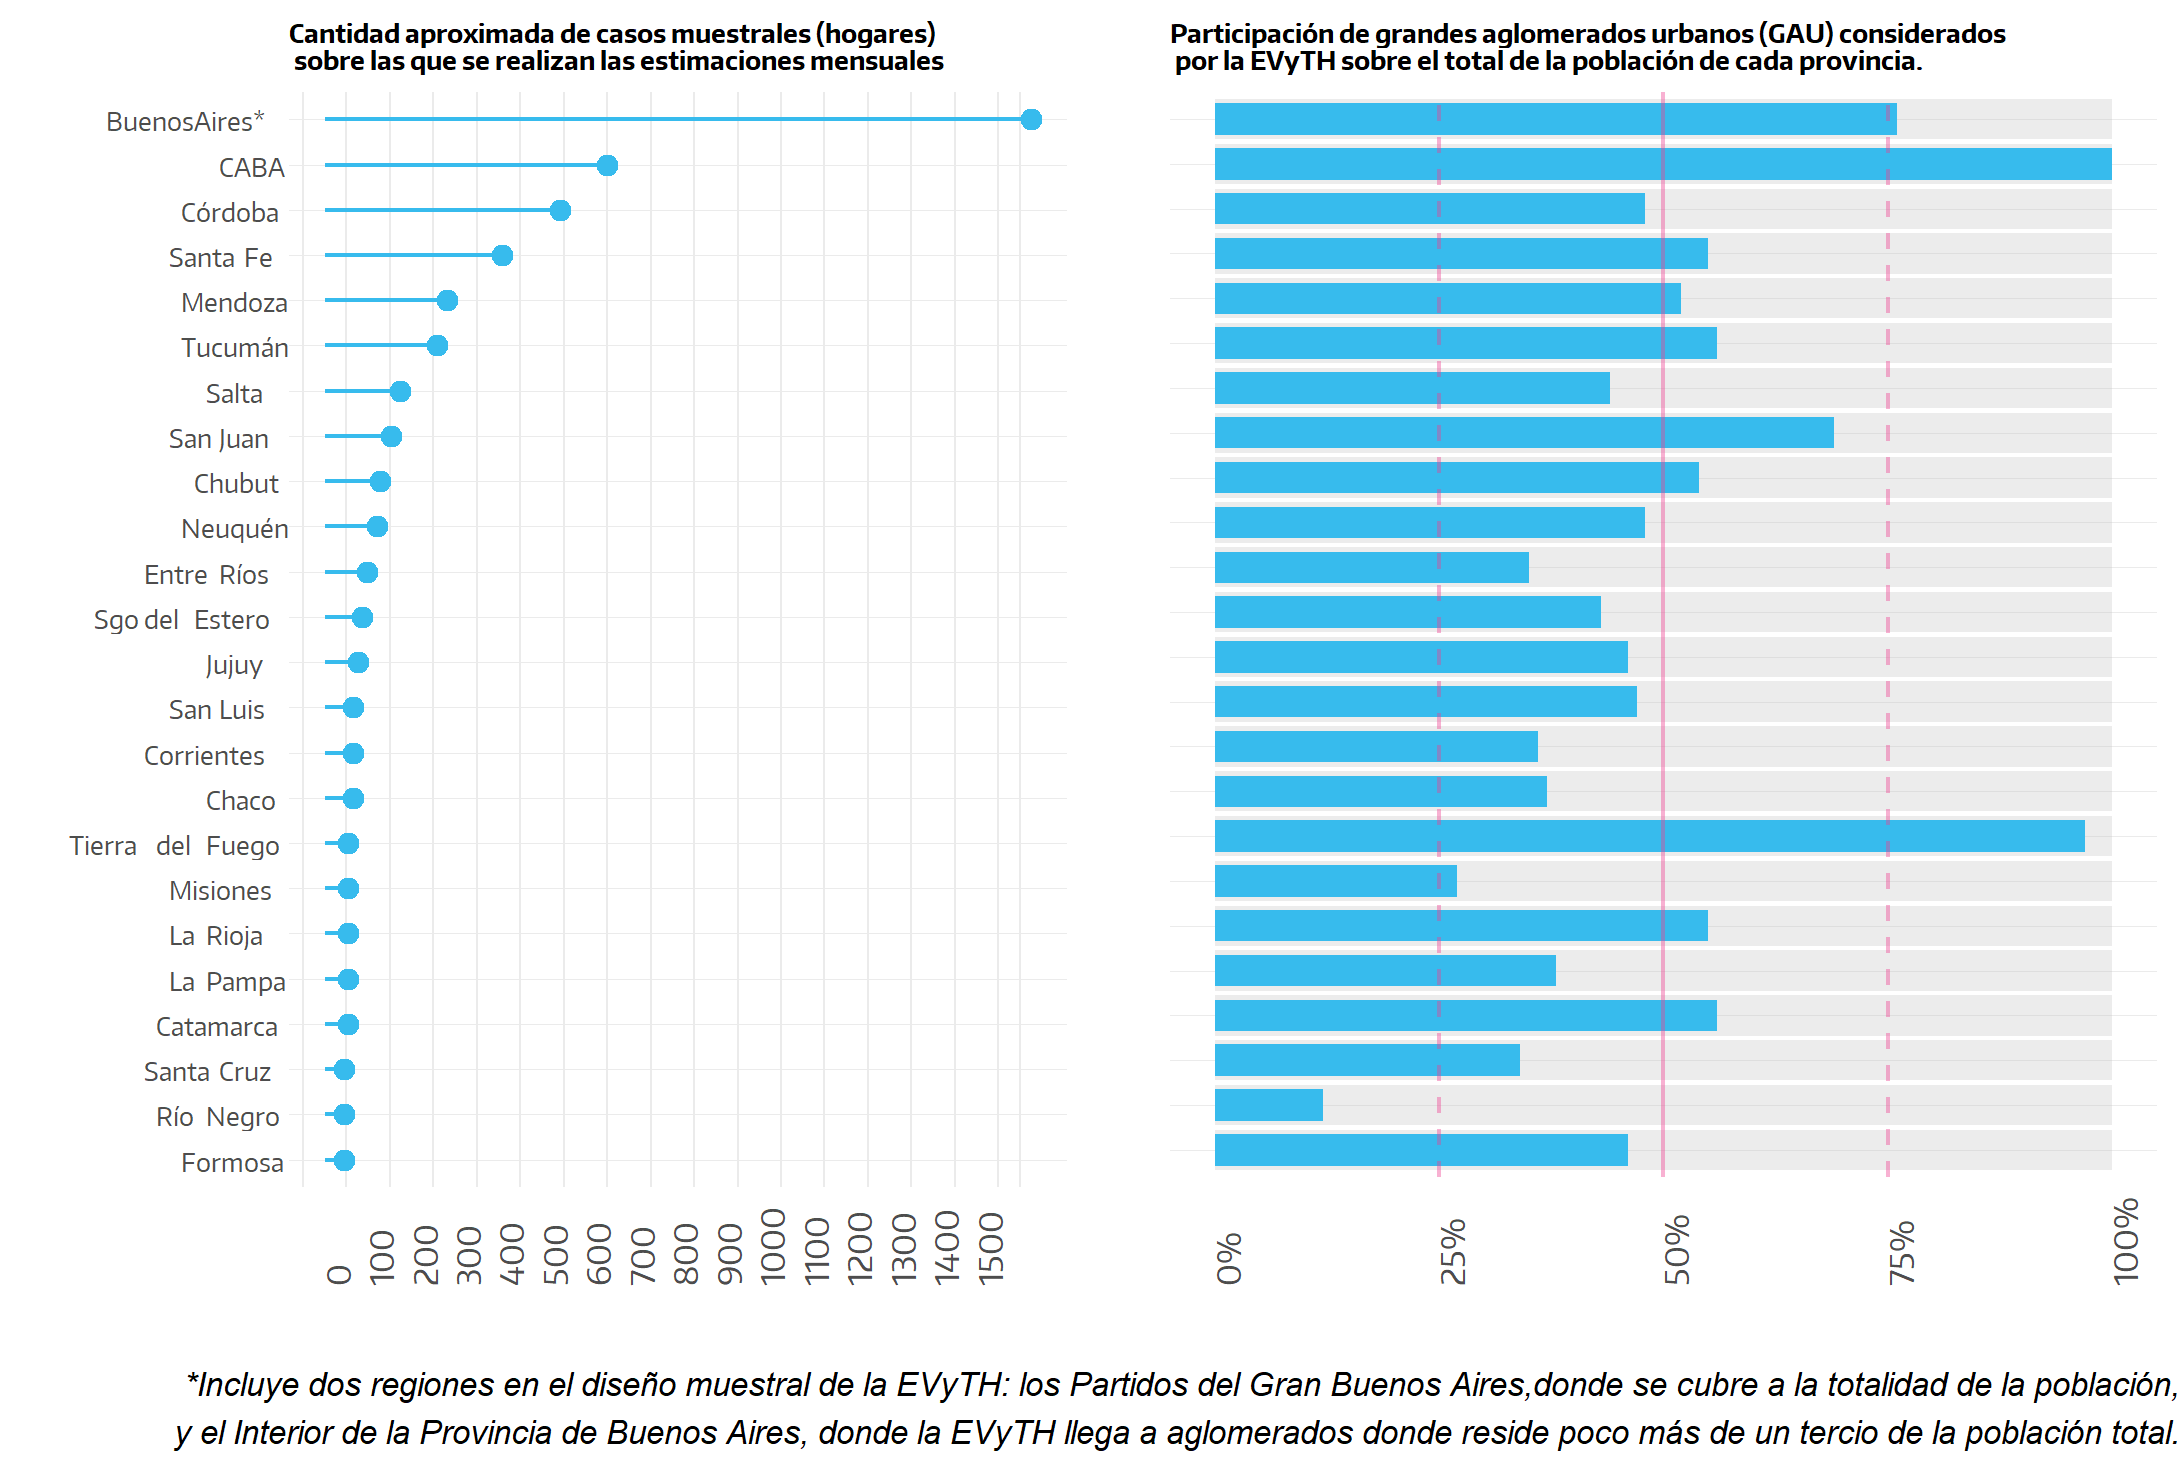
\includegraphics[width=0.8\linewidth]{imagenes/figura2.1} 

}

\caption{Cantidad y participación}\label{fig:cantidades}
\end{figure}

Para más información de la EVyTH podes consultar los informes técnicos de resultados y las series estadísticas en:

\href{http://datos.yvera.gob.ar/dataset/encuesta-viajes-turismo-hogares-evyth}{Data abierta}

\href{https://www.yvera.tur.ar/estadistica/info/encuesta-de-viajes-y-turismo-de-los-hogares-evyth}{Informes técnicos}

\href{https://www.indec.gob.ar/indec/web/Institucional-Indec-OperacionesEstadisticas}{Encuesta Permanente a Hogares del INDEC}

\hypertarget{eoh}{%
\section{EOH}\label{eoh}}

La \textbf{Encuesta de Ocupación Hotelera (EOH)} es un relevamiento realizado en forma continua desde el 2004, bajo la \href{https://www.indec.gob.ar/indec/web/Nivel4-Tema-3-13-56}{coordinación del MINTURDEP y el Instituto Nacional de Estadísticas y Censos (INDEC)}, que tiene como objetivo medir el impacto del turismo interno e internacional sobre la actividad de los establecimientos hoteleros y para-hoteleros.
Con periodicidad mensual, mide, entre otras variables, la cantidad de pernoctes, de viajeros residentes y no residentes, la estadía promedio por viajero y la tasa de ocupación en plazas y habitaciones.
Además, permite distinguir la información de acuerdo al origen de los viajeros (provincia o país de residencia).

Este operativo releva 49 de las localidades con mayor oferta hotelera y para-hotelera del país, dentro de las siete regiones turísticas definidas por el MINTURDEP.
Por tanto, su cobertura respecto a la contabilización del turismo se debe considerar desde el punto de vista del destino del viaje (independientemente del origen o lugar de residencia del viajero).

Cabe señalar que, como muestra la Figura \ref{fig:cobertura}, el peso de las localidades incluidas en este estudio sobre el total del sector hotelero y parahotelero de cada provincia muestra importantes diferencias entre las mismas.

\textbf{Figura 2.2. Cobertura de la EOH. Porcentaje aproximado que representan las plazas de las localidades incluidas en la EOH respecto al total de plazas hoteleras y parahoteleas provinciales. Datos a diciembre de 2019.}

\begin{figure}

{\centering 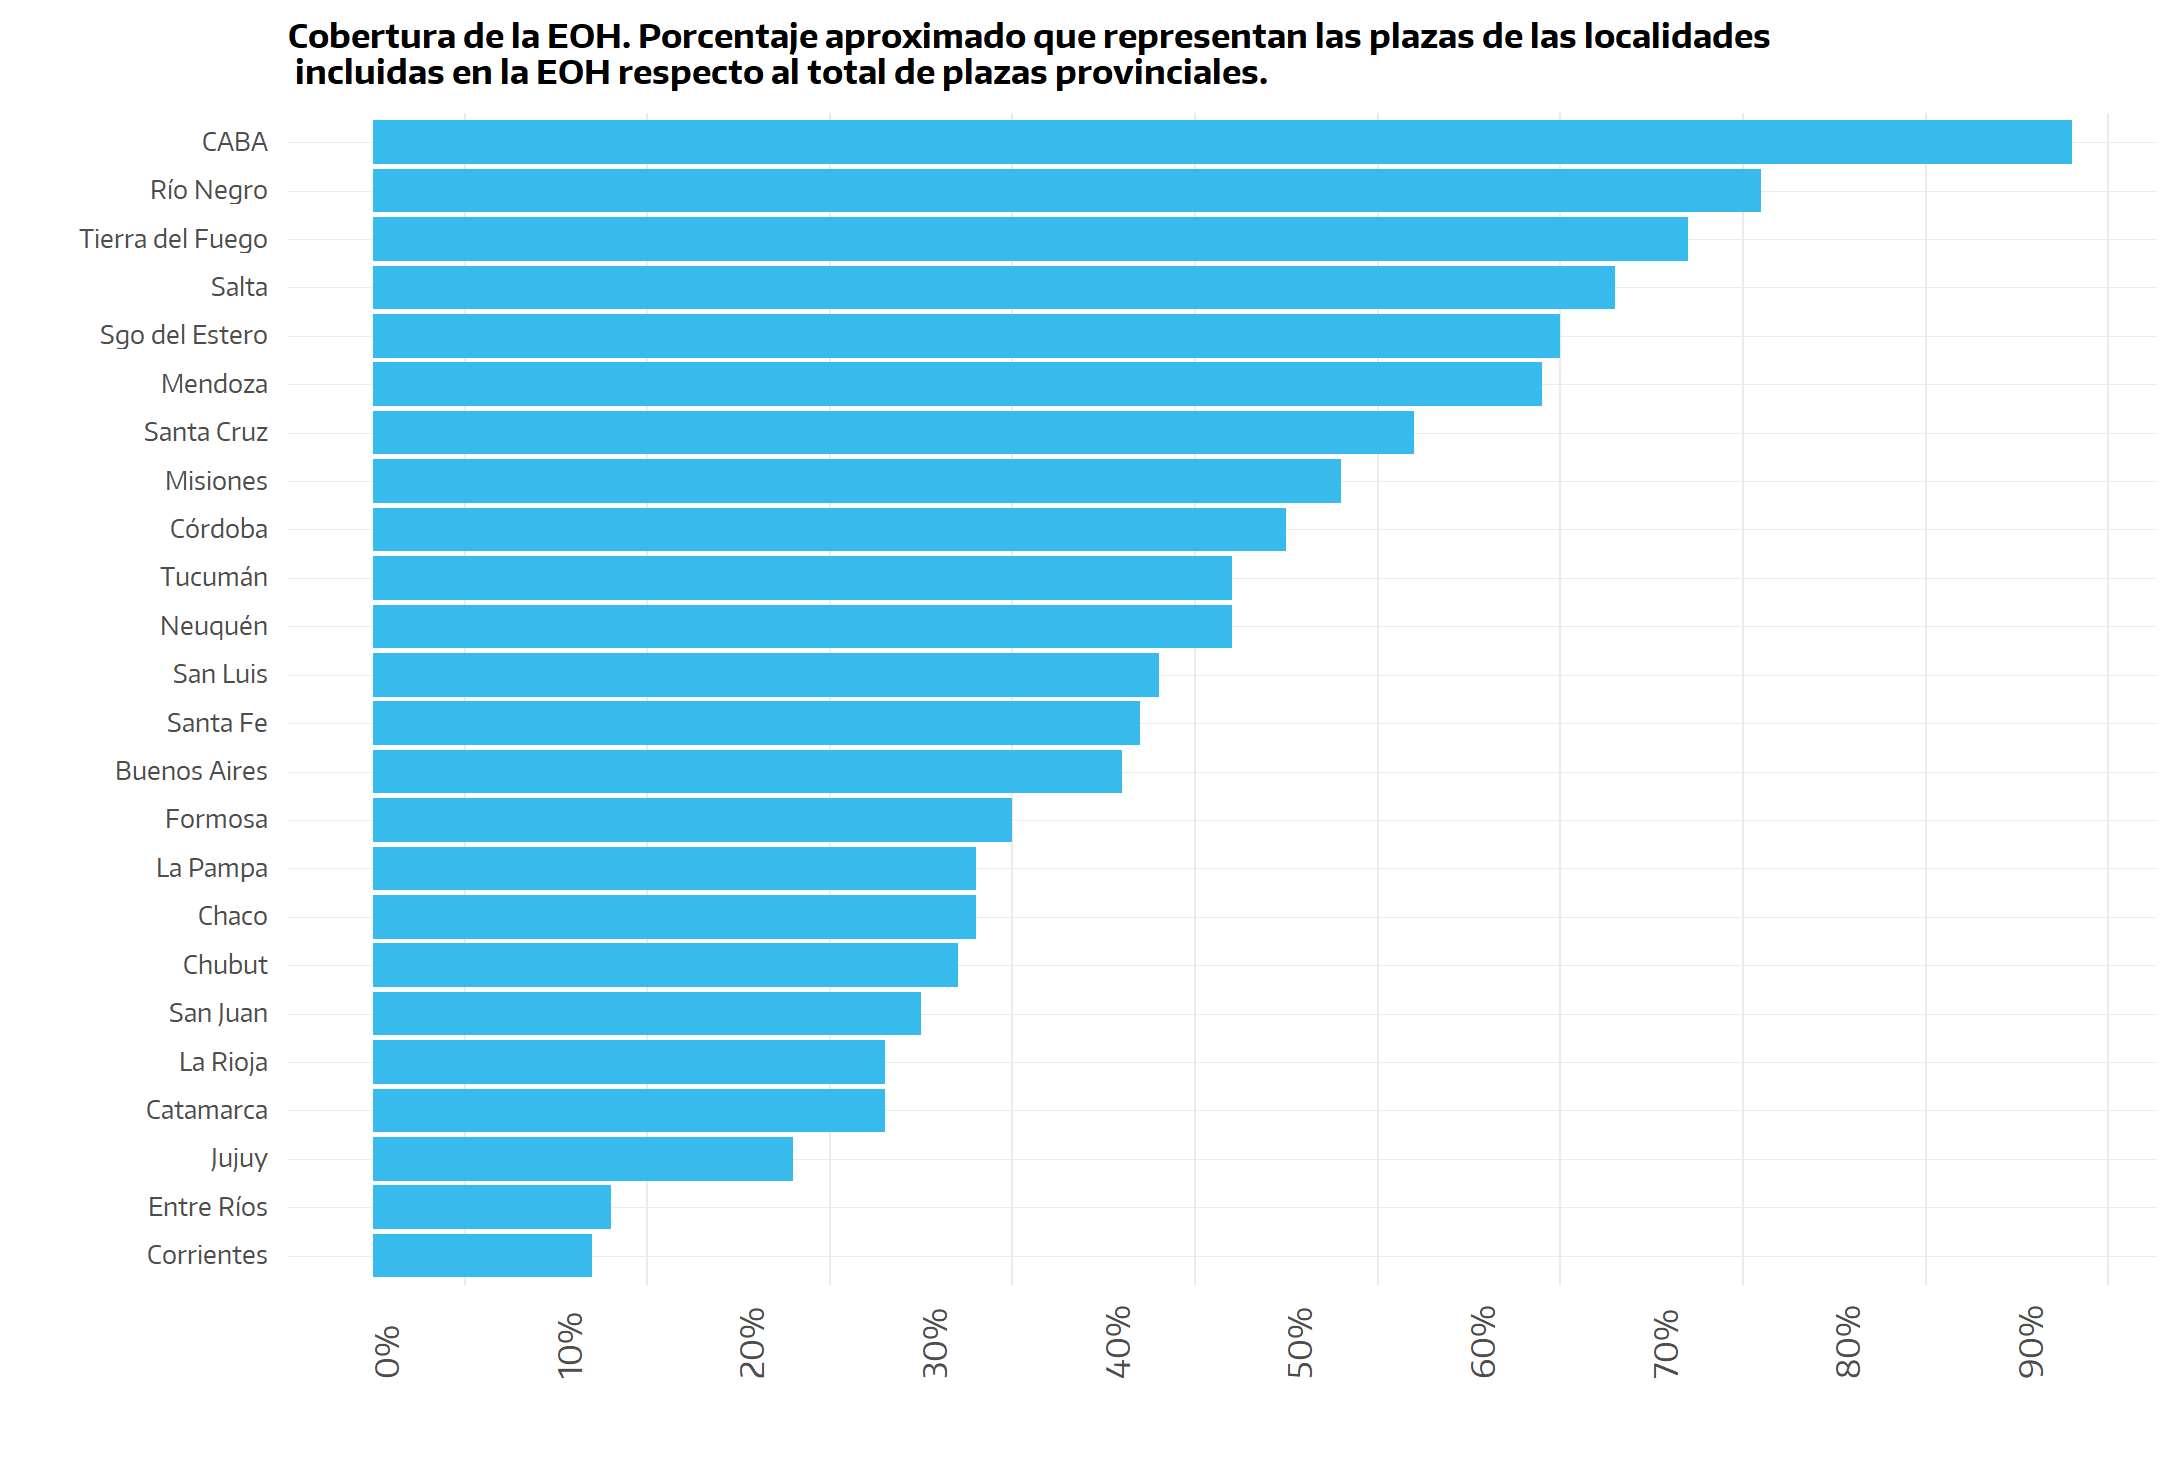
\includegraphics[width=0.8\linewidth]{imagenes/figura2.2} 

}

\caption{cobertura de la EOH}\label{fig:cobertura}
\end{figure}

Los tipos de establecimientos incluidos en la muestra son, dentro de los hoteleros, los hoteles de 1 a 5 estrellas y los apart-hoteles; y, dentro de los para-hoteleros, los hoteles sindicales, albergues, cabañas, bungalows, hospedajes, bed \& breakfast, hosterías, etc.
Cabe señalar que la EOH excluye de su universo a los establecimientos pequeños (menos de 4 habitaciones o de 12 plazas inclusive).

Todos los viajeros que se alojen en estos tipos de establecimientos dentro de las localidades consideradas, serán relevados por la encuesta.

Sin embargo, además de las localidades no incluidas en el diseño muestral de la encuesta, cabe recordar que, aún en las localidades consideradas, quedan por fuera del operativo las viviendas de alquiler temporario y los campings, así como también las segundas viviendas y las viviendas de familiares y amigos, y otros lugares de alojamiento de menor relevancia.
Por otro lado, considera solamente a las personas que pernoctaron en el destino, dejando fuera a los excursionistas.

Asimismo, al analizar viajeros hospedados (o huéspedes), a partir de la informacion brindada por los hoteleros, no es posible que se distingua, dado la dificultad de su clasificación, entre los visitantes y los otros viajeros alojados en los establecimientos.

Para más información de los informes de resultados, series estadísticas y la metodología, vistá:

\href{https://www.yvera.tur.ar/estadistica/info/encuesta-de-ocupacion-hotelera-eoh}{Informes de prensa en Yvera}

\href{http://datos.yvera.tur.ar/dataset/encuesta-ocupacion-hotelera-parahotelera-eoh}{Data Abierta}

\href{https://www.indec.gob.ar/ftp/cuadros/economia/eoh_aspectos_metodologicos.pdf}{Doc metodológico (INDEC)}

\hypertarget{eti}{%
\section{ETI}\label{eti}}

La \textbf{Encuesta de Turismo Internacional (ETI)} es otro operativo realizado en forma continua desde el año 2004, \href{https://www.indec.gob.ar/indec/web/Nivel4-Tema-3-13-55}{coordinado conjuntamente por el MINTURDEP y el INDEC}.

Tiene por objetivo general conocer las características de los viajes (el motivo, la duración, el/los destino/s, el/los tipos de alojamientos utilizados, etc.), y de los viajeros (lugar de residencia, conformación del grupo viajero, etc.), así como los gastos en alojamiento, alimentación, traslados, transportes y compras que realizan los viajeros en los lugares visitados.

Releva a los viajeros no residentes en la Argentina que visitaron el país (al salir del país) y a los viajeros residentes en Argentina que viajan al exterior (al volver al país).

Cubre el movimiento internacional de seis puntos de entrada y salida del país: Aeropuerto de Ezeiza, Aeroparque Jorge Newbery, Aeropuerto de Córdoba (Pajas Blancas), Aeropuerto de Mendoza (El Plumerillo), Puerto de Buenos Aires y el paso fronterizo terrestre Sistema Cristo Redentor, que representan aproximadamente la mitad del flujo internacional de viajeros, dejando fuera de análisis los ingresos y egresos por otros puntos de frontera.
En este sentido, es preciso tener en cuenta que el comportamiento y las características de los viajes de quienes ingresan o egresan por los puntos de acceso cubiertos por la encuesta, es diferente al de los viajeros que lo hacen por otros puntos.

A partir del año 2019 la pregunta de los destinos visitados (itinerario) en Argentina es de tipo abierta y se registra todos aquellos lugares donde el turista realiza al menos una pernoctación junto con el tipo de alojamiento utilizado.
Hasta el año 2018 la encuesta contemplaba 13 destinos principales (localidad o zona o provincia, según el caso) y una categoría que engloba a todos los destinos regionales no contemplados entre los anteriores.
Por esta razón, los datos históricos, en la mayoría de los casos, no se encuentran disponibles con apertura provincial.

\hypertarget{suxedntesis}{%
\section{Síntesis}\label{suxedntesis}}

\textbf{Principales características y cobertura de las Encuestas Nacionales de Turismo}

La Figura \ref{fig:ent} presenta en forma comparativa las principales características de cada una de las tres Encuestas Nacionales de Turismo (ENT) que releva el MINTURDEP.

\begin{figure}

{\centering 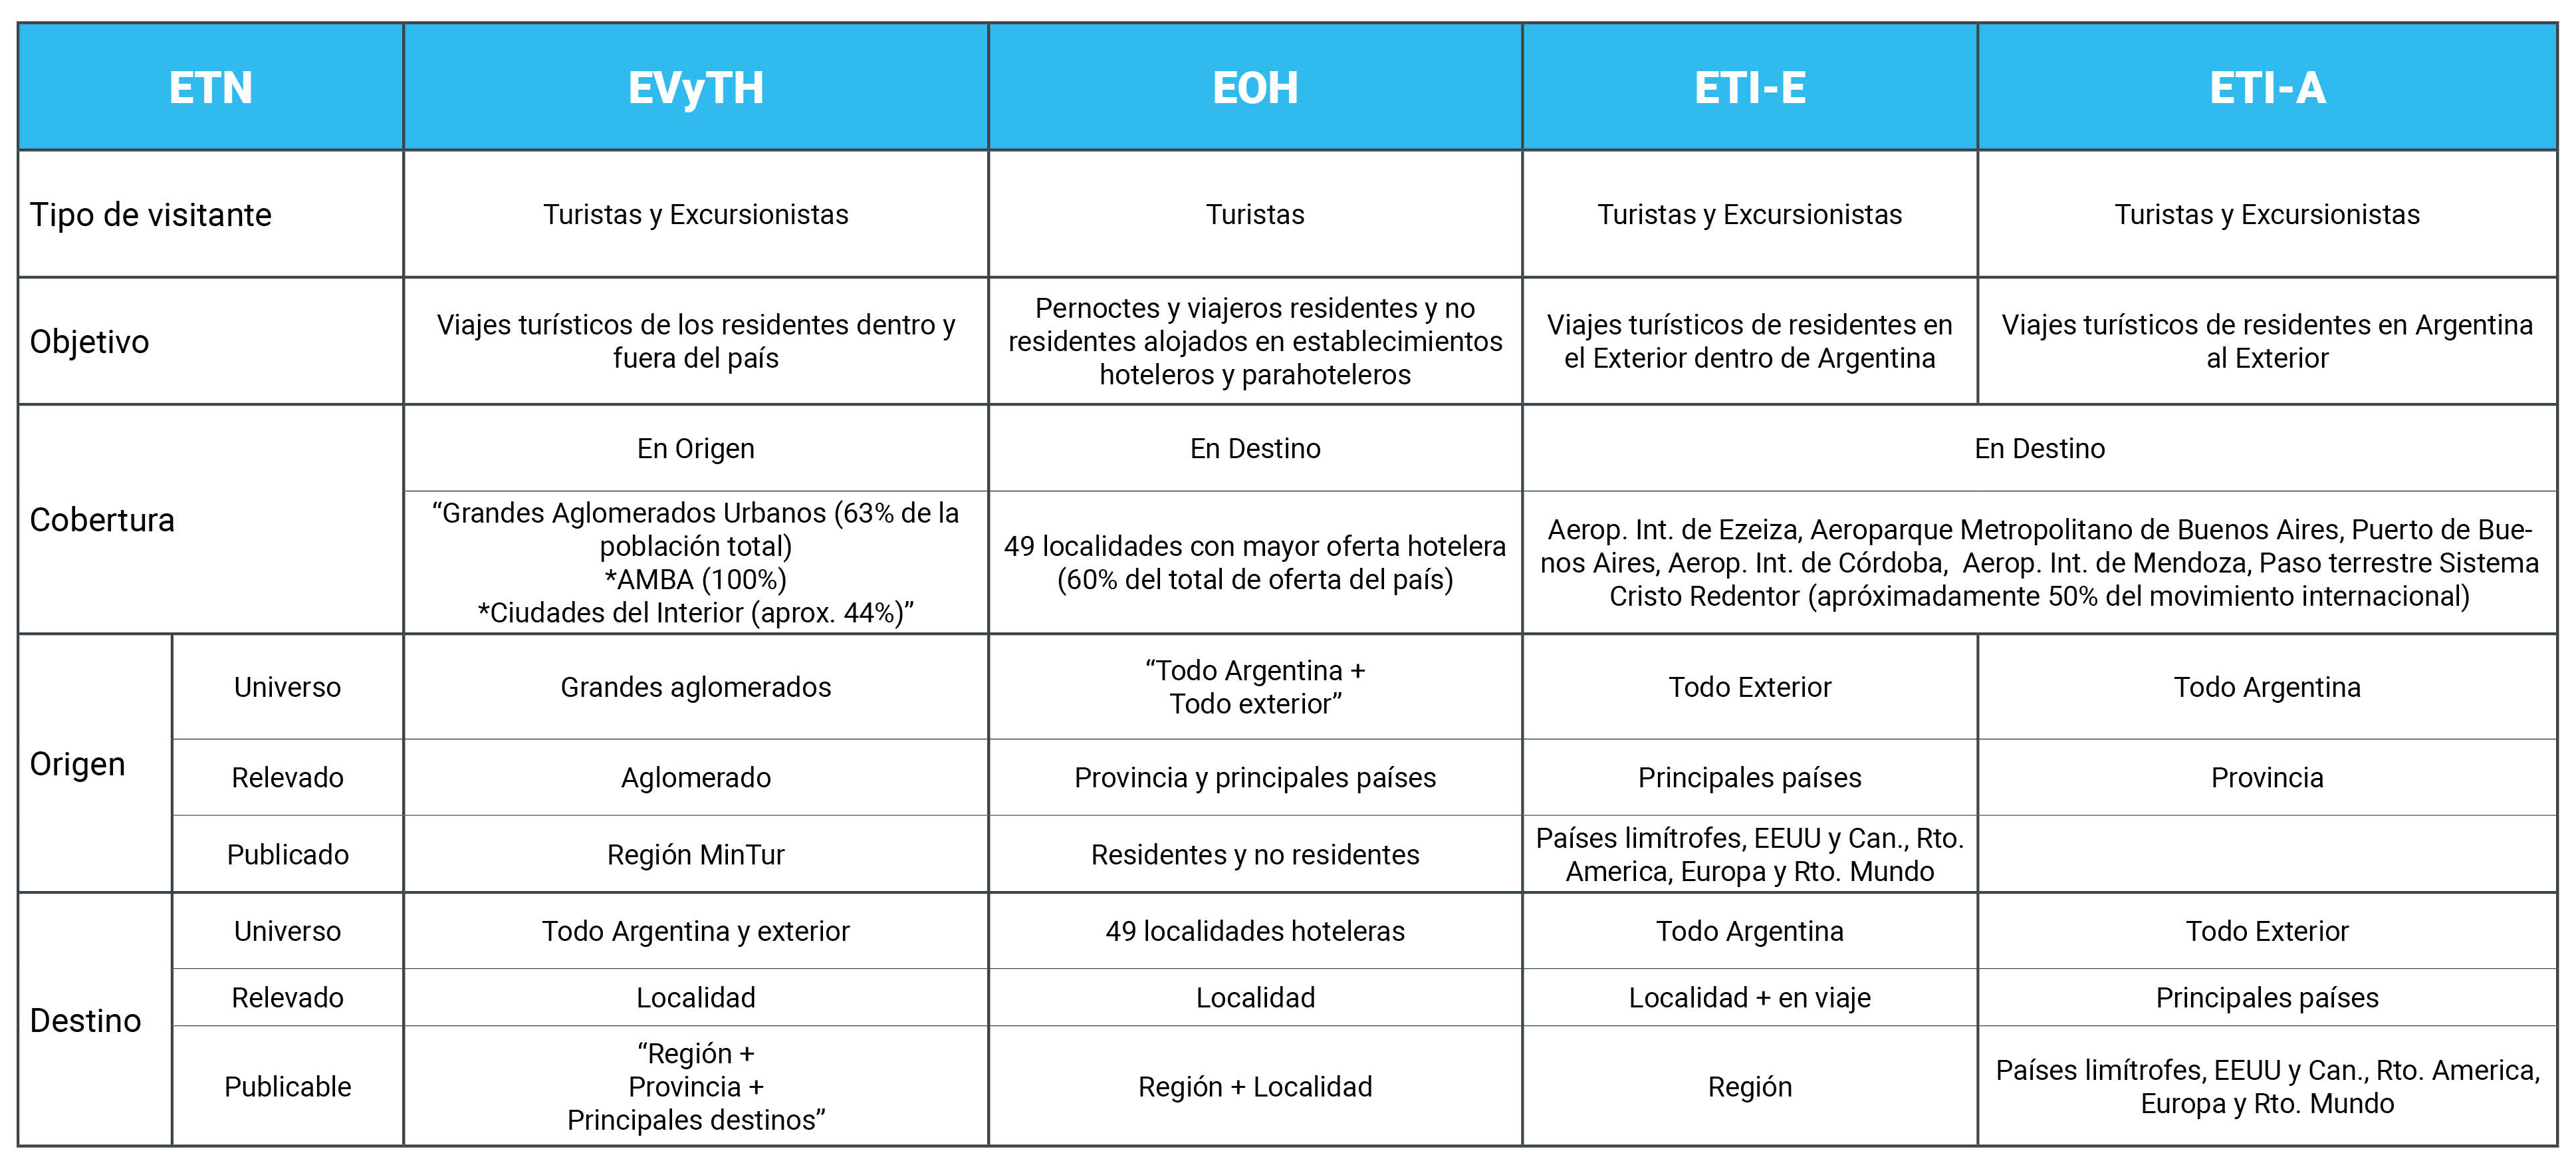
\includegraphics[width=0.8\linewidth]{imagenes/figura2.3} 

}

\caption{Principales características de las Encuestas Nacionales de Turismo (ENT)}\label{fig:ent}
\end{figure}

Asimismo, la Figura \ref{fig:coberturaENT} da cuenta de cuáles son los segmentos de visitantes de los que se puede dar cuenta ``teóricamente'' (sin entrar en el análisis de la robustez de las estimaciones, más aún considerando niveles provinciales) a partir de estos estudios.
Como puede observarse, hay una importante cantidad de segmentos (sombreados en rojo) para los que ninguna fuente actualmente puede brindar información.

\begin{figure}

{\centering 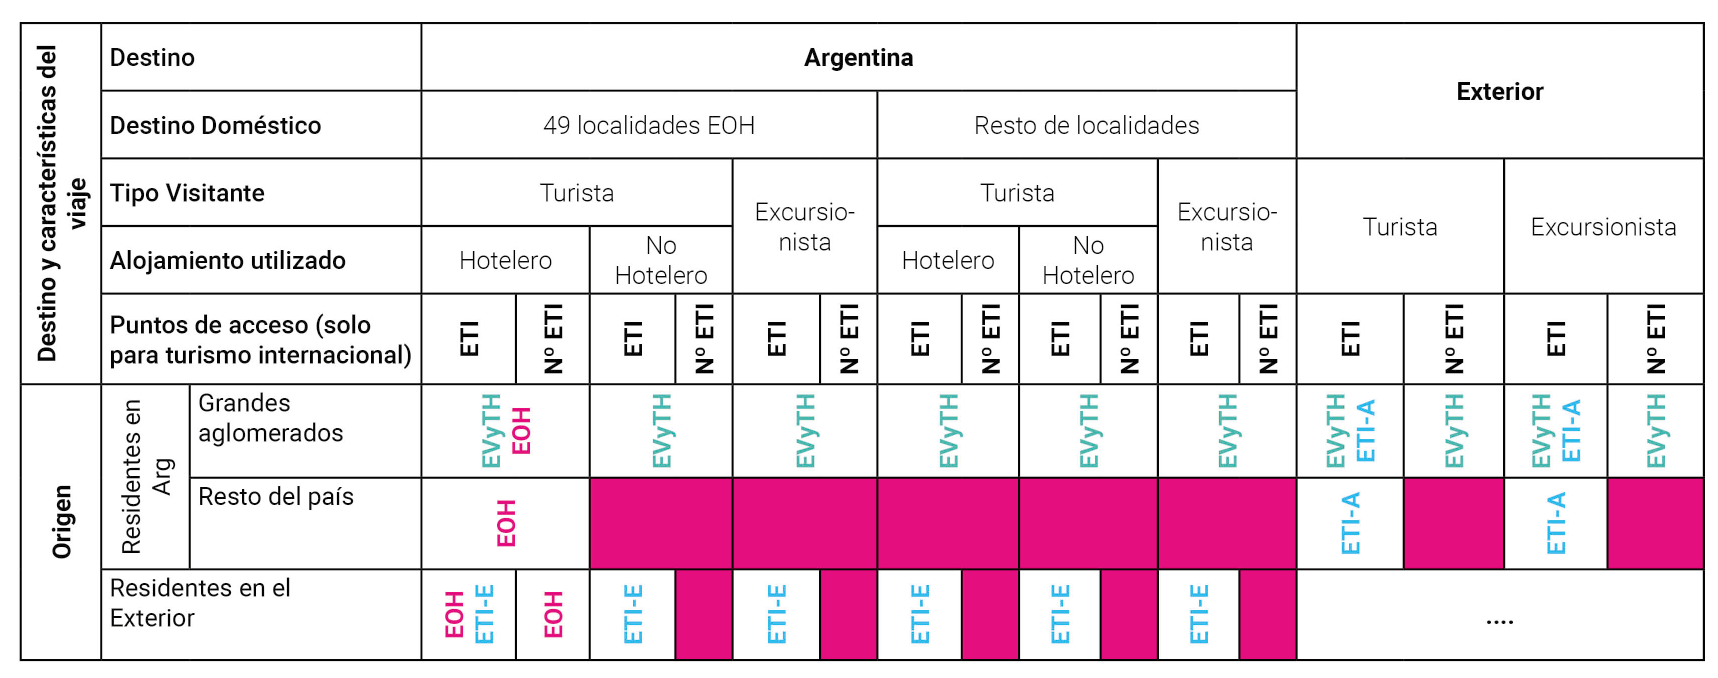
\includegraphics[width=0.8\linewidth]{imagenes/figura2.4} 

}

\caption{Cobertura teórica por parte de las ENT de los visitantes según origen y destino.}\label{fig:coberturaENT}
\end{figure}

Para ver un ejemplo de cómo el MINTURDEP utiliza los datos de estas encuestas para obtener resultados a nivel de provincia se pueden visitar las fichas de ``\href{https://www.yvera.tur.ar/estadistica/info/estadisticas-de-turismo-por-provincias}{Estadísticas de turismo por provincia}''.

\hypertarget{consideraciones-finales}{%
\chapter*{Consideraciones Finales}\label{consideraciones-finales}}
\addcontentsline{toc}{chapter}{Consideraciones Finales}

Este documento de trabajo pretende plantear la importancia de las definiciones conceptuales y de la rigurosidad metodológica (es decir la forma en que esos conceptos se operacionalizan, se hacen medibles) para la producción de información estadística rigurosa.

El turismo constituye un fenómeno harto complejo de mensurar, con lo cual lo antedicho cobra especial relevancia.
Sólo garantizando un mismo marco conceptual y opciones metodológicas consistentes (lo que implica no necesariamente diseños perfectos, muchas veces inalcanzables, aunque sí un conocimiento pleno de sus limitaciones) será posible alcanzar indicadores básicos de estadística de turismo (nacionales, provinciales e incluso municipales) robustos y comparables.

Lo expuesto revela, entonces, la necesidad y la importancia de lograr una interrelación continua y eficaz entre los diferentes niveles de producción de estadística de turismo.

  \bibliography{book.bib,packages.bib}

\end{document}
